% !Mode:: "TeX:UTF-8"
\baselineskip 20pt


\chapter{基于深度生成模型的动态网络社团检测大规模扩展}
\label{chap:6}

随着网络表示学习的快速发展,生成模型对网络拓扑的解耦以及对网络语义信息的聚合大大降低了大规模网络的计算复杂度,逐渐替代了现有的矩阵分解、概率图模型等方法对网络进行直接建模的方法。然而其基于图神经网络的深度学习方法对网络的建模是黑盒建模,即其模型中的参数并不具备现实或物理意义,而其强大的拟合能力能够较好地刻画节点的拓扑与属性信息,间接支撑复杂网络的下游任务效果,但难以为动态网络演化模式分析、网络功能结构挖掘等提供帮助。因此,本章提出基于深度生成模型的动态网络建模方法(VGRGMM),通过变分自编码器架构,结合深度序列模型建模动态网络,引入混合高斯先验来同时计算动态网络的社团结果,即提升了模型的运行效率,也为后续网络演化分析提供了可解释的中间参数用以支撑对动态网络的后续挖掘。在真实世界数据和生成数据的大量实验表明,VGRGMM模型在社团检测及社团演化分析任务中都表现出优于对比方法的效果,证明了VGRGMM模型可以在结合深度学习模型框架与生成模型的结合中融合二者的优点。



\section{引言\label{chap6:intro}}


动态网络由于其能够建模许多现实世界的复杂系统,长期以来一直受到研究者的关注,其能够建模包括社交网络中的人员关系~\cite{newman2004finding}、学术论文之间的引用关系与合作关系~\cite{gopalan2013efficient,chikhaoui2015new}以及生物网络如蛋白质-蛋白质相互作用关系~\cite{palla2005uncovering,zhang2019relational}等。动态社团检测旨在发现隐藏在动态网络中的有意义的群体或簇~\cite{7384503,rossetti2018community},这对信息传播~\cite{del2016spreading}、链接预测~\cite{lu2015toward,yu2017link,Ma.2019.Ming}等多种应用及动态网络规律\cite{laurienti2009modularity}挖掘都具有重要意义。另外,作为动态社团检测的一个重要组成部分,社团演化分析则侧重于分析社团及网络在时序演化过程中的模式,还可以揭示网络的演化特征,量化连续快照之间社团的过渡关系~\cite{tang2014detecting}。因此,动态网络社团检测通过显式或隐式地建模动态网络的演化可以更好地模拟真实的复杂系统,并且相比于静态网络中的社团检测具有更多的挑战~\cite{rossetti2018community}。


许多工作已经被提出用于检测动态网络中的社团结构并分析其演化,例如模块度优化算法~\cite{Mucha.2010.Onnela}、谱聚类算法~\cite{liu2018global}、多目标优化算法~\cite{Zhang.2017.Niu,Zhang.2020.Jin}、非负矩阵分解算法~\cite{Ma.2017.Dong}和生成模型~\cite{pensky2019spectral}等等。上述方法各有优点,但对于动态网络演化建模的设计大部分是通过添加额外的惩罚项来实现对相邻网络快照的平滑性约束,部分方法如生成模型可以通过设计动态网络的演化机制实现对动态网络演化模式的显式建模,然而此类方法大部分设计较复杂,因此无法适应于大规模网络,且其模型参数求解方法存在一定门槛,往往难以大规模应用与推广。
% 动态随机块模型和隐空间模型是解决该问题的两种生成方法。所有这些时间社团检测方法都是专门设计的,并且各有其优点。


近年来,作为深度学习的重要分支~\cite{Sun.2021.Xu},网络表示学习在复杂网络分析中取得了广泛的成功~\cite{8476241,Liu.2021.Lv}。网络表示学习将网络中的每个节点嵌入到低维空间中,实现对网络中节点之间复杂依赖关系的解耦,使得网络大部分下游任务得以更高效地执行,如节点分类、异常节点识别和链接预测等。对网络表示学习方法的研究也存在多种技术路线,包括矩阵分解、随机游走和图神经网络等~\cite{zhang2018network,perozzi2014deepwalk,grover2016node2vec,tang2015line,wang2016structural}。另外,一些基于社团的网络表示学习方法在静态网络中表现出色,社团结构的引入能够帮助网络表示学习方法整合节点拓扑和属性信息以提高潜在表示的能力,而网络表示学习也提升了模型对社团检测任务的执行效果~\cite{cavallari2017learning,choong2018learning,shi2019network,jin2019community}。



然而,上述方法多是为静态网络设计的,并未建模网络的演化机制。为了提取动态网络的丰富时间信息,也有研究人员提出了新方法以实现在动态网络表示学习方法中建模动态网络的演化模式~\cite{goyal2020dyngraph2vec,trivedi2017know,7880588,zhou2018dynamic,Yang.2020.Shen,pareja2020evolvegcn}。例如,VGRNN~\cite{hajiramezanali2019variational}将高维的随机变量融合到图递归神经网络中,以学习可解释的潜在表示并生成动态网络,所学习的表示向量也可以用于预测网络中未来的边。关于动态网络表示学习的全面综述可以参考~\cite{jmlr:v21:19-447}。
通常,动态网络表示学习所得到的节点表示,可以进一步通过无监督聚类算法获得社团结构。但这种两步法可能会得到错误的社团结果,因为其表示向量的学习并没有考虑到网络中存在的社团信息。这涉及到网络中社团的基本定义,基于图神经网络的动态网络表示学习方法虽然将节点属性与拓扑特征均映射到了节点表示向量中,但考虑到图神经网络本身设计会过滤掉网络中的高频信息,这使得节点表示若没有社团结构的融入将无法准确识别网络中紧密连接的连通子图,即普遍意义上的社团结构。因此,建模能够建模社团拓扑结构变化的动态网络表示学习方法是必要的。然而,动态网络表示学习方法融入社团信息面临着诸多挑战,例如动态网络中边的动态变化、节点表示向量的演化对边生成的影响以及动态社团结构对节点表示向量的影响等均需要解决。



为了解决上述挑战,本章尝试基于动态网络表示学习架构来建模具有社团结构的动态网络,并利用动态网络表示学习方法来增强动态社团检测任务。首先,上述问题可以从概率的角度加以解决,而非采用两步法,因其忽略了建模过程中的不确定性且基于表示向量的聚类结果无法完全契合社团结构。本方法假设节点和边的形成与其所在社团有关,而节点的社团归属服从混合高斯分布(GMM),这有助于将社团检测和网络表示学习耦合到一个联合概率分布中。其次,该方法有助于捕捉常见网络的网络特征,从而更好地理解现实世界中的网络,通过将变分自编码器(VAE)~\cite{kingma2013auto}中的单一先验替换为社团混合高斯先验,可以改进每个动态网络快照中的社团检测效果,并且社团结果可以帮助提升节点表示学习效果。此外,循环神经网络(RNN)~\cite{lipton2015critical}能够高效地捕获时序信息,其已广泛应用于序列数据的建模中,本方法受RNN启发,也考虑利用深度序列模型隐式地刻画网络的演化模式。与以往动态网络建模中的其他方法不同,本方法将RNN整合到概率模型中,使社区检测和演化建模更加合理。具体来说,本方法针对节点间时序演化模式构建了门控循环单元结构(GRU),来捕获节点表示向量所在的高维空间中的复杂时序依赖关系。

总而言之,本章提出了一种名为VGRGMM的动态社团检测模型,该模型融合了变分图自编码器、门控循环单元和高斯混合模型。作为一个端到端的框架,VGRGMM可以同时实现对动态网络表示学习任务和动态社团检测任务的互增强。本方法的主要贡献总结如下:
\begin{itemize}
    \item[$\bullet$] 本研究提出了一种基于图深度学习的无监督动态社团检测模型VGRGMM,该模型能够有效地建模动态社团结构和动态网络表示学习。
    \item[$\bullet$] 所提出的模型将动态网络快照中的社团整合到一个带有混合高斯先验的变分自编码器中,并结合GRU捕获向量空间中的时序演化模式。
    \item[$\bullet$] 在大量真实数据中的实验结果表明,与对比方法相比,VGRGMM在生成数据集和真实世界网络上的动态社团检测性能具有显著提升。针对真实数据的样例分析结果也证明了VGRGMM方法相较于对比方法具有更优的社团检测效果,并能够有效地刻画动态社团的演化模式。
\end{itemize}


\section{VGRGMM模型描述\label{chap6:model}}

% \label{sec:method}
%=============Figure1 VGRGMM==============
\begin{figure*}
\centering 
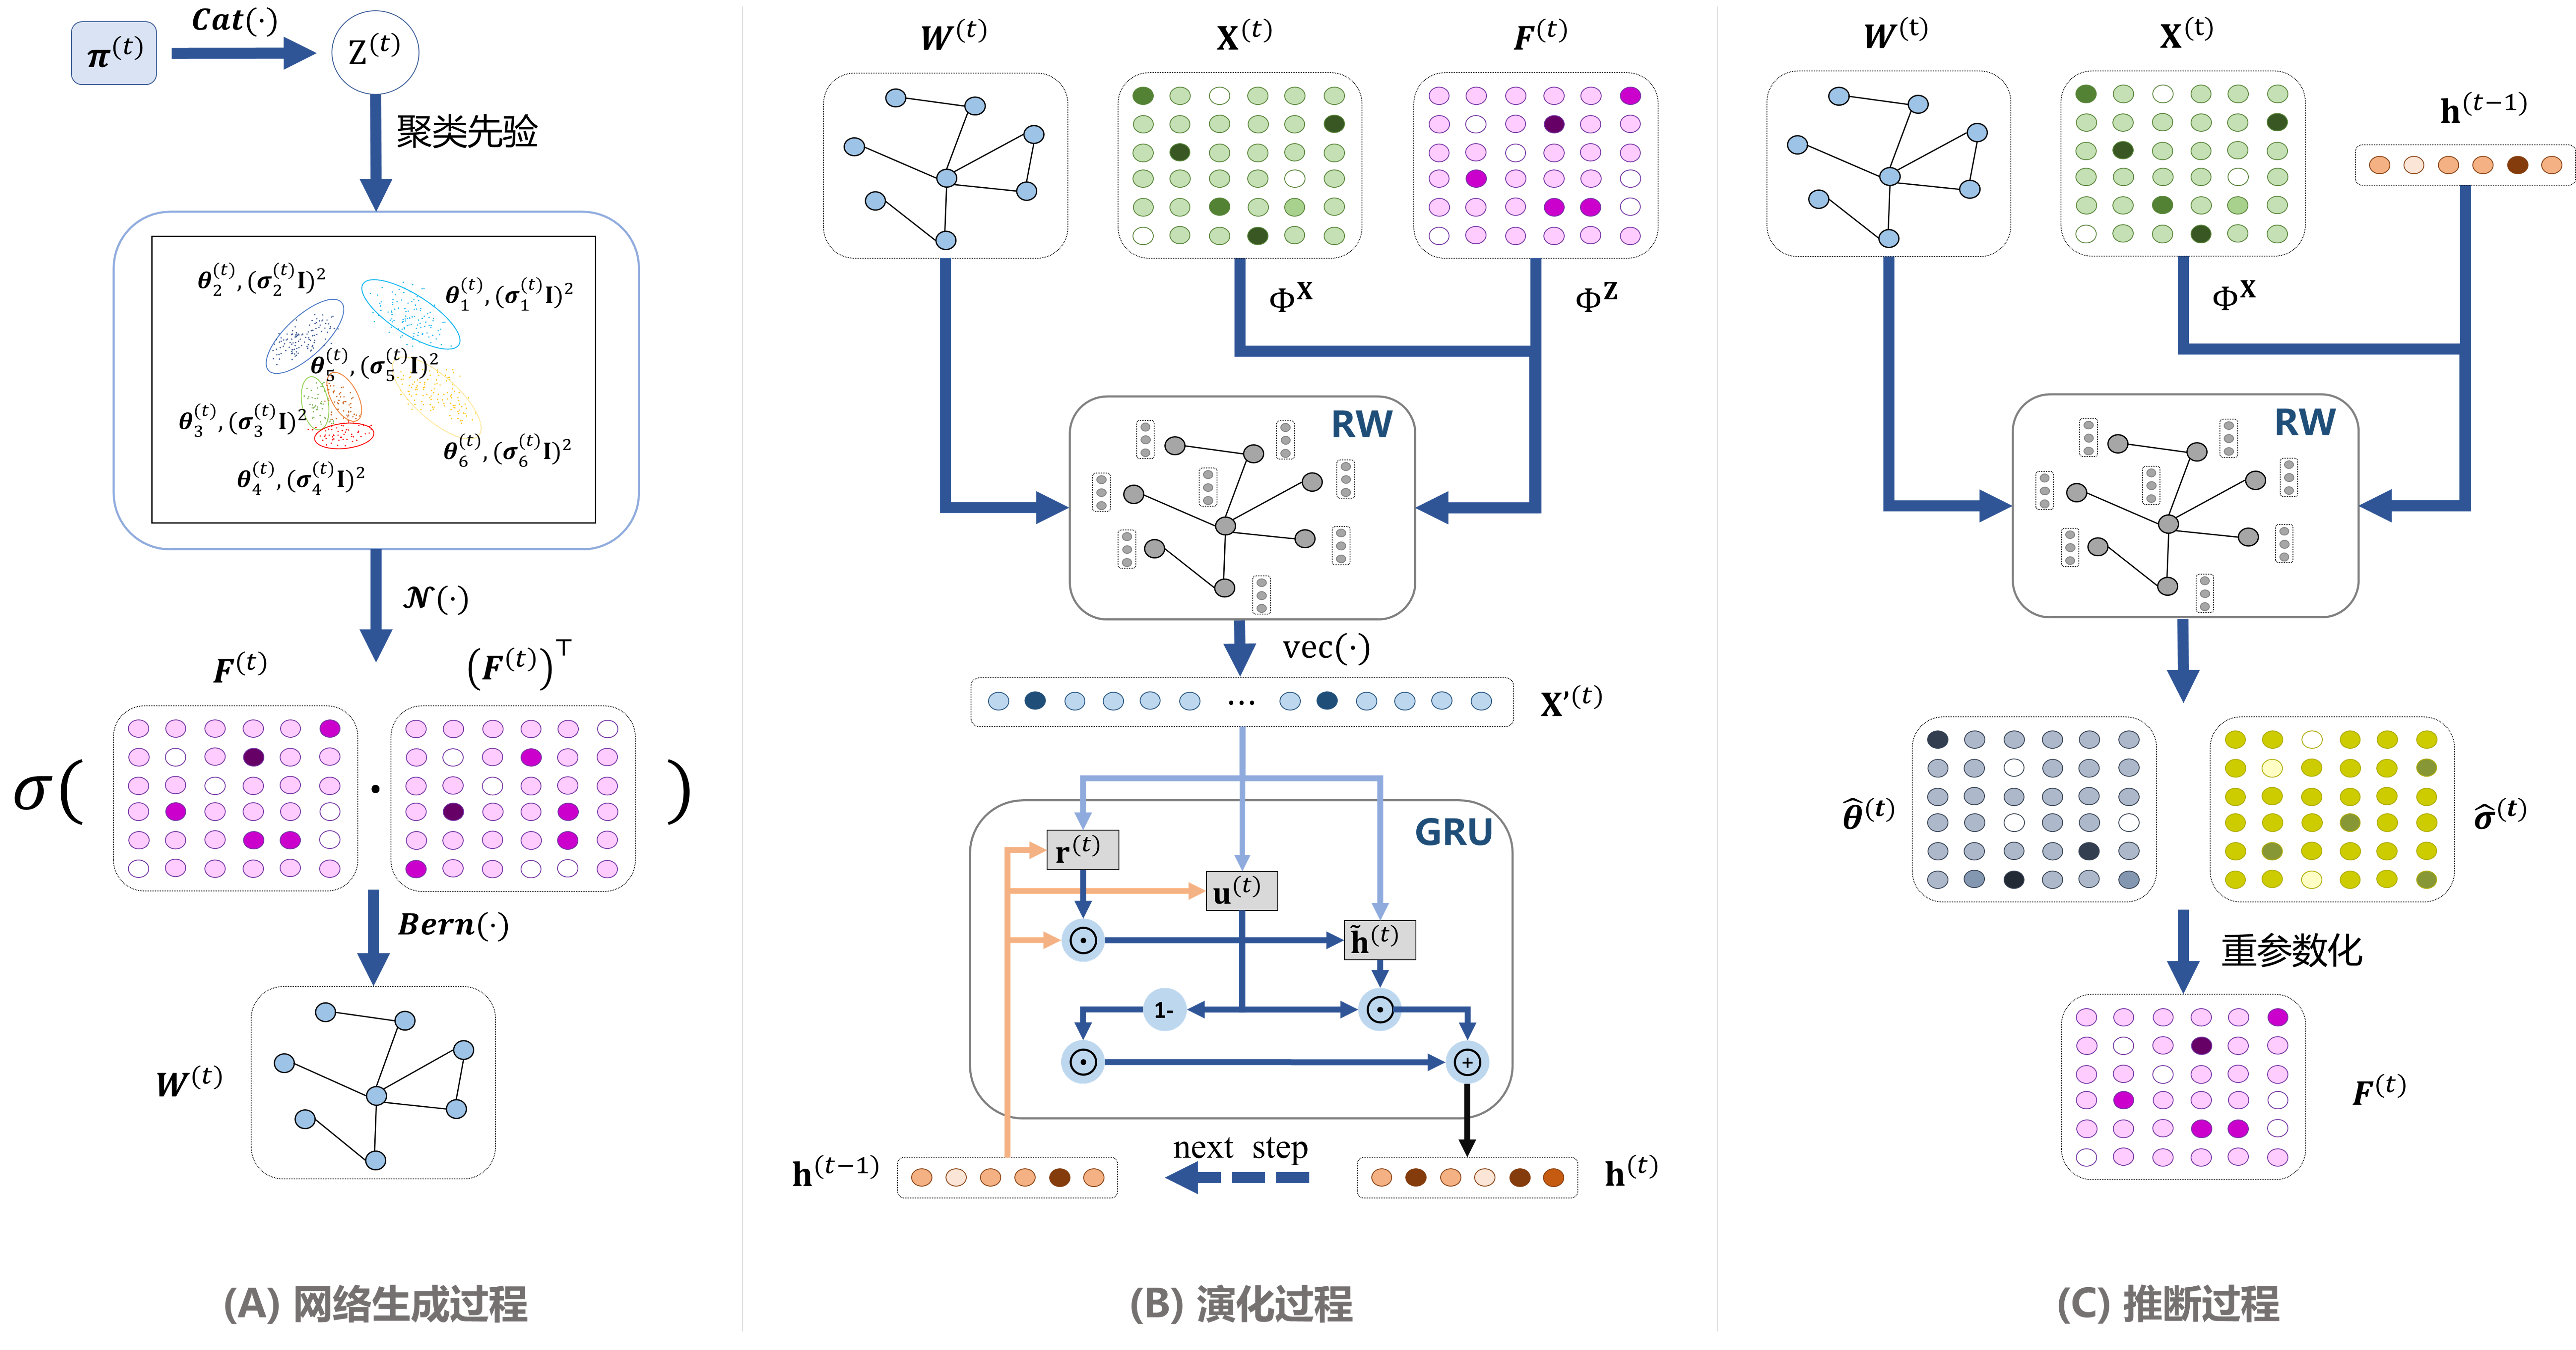
\includegraphics[width=\textwidth]{figures/chap06/VGRGMM.png}
\caption{VGRGMM框架在快照$t$上的工作流程
} 
\label{fig1}
%\vspace{-0.2cm}
\end{figure*}


本节首先介绍本章所使用的符号及其定义,随后介绍本章所提出的VGRGMM模型框架及其详细过程以及模型的推断方法。

\subsection{符号与问题定义}
本研究主要关注无向无权的动态网络,记为$\mathcal{G}=\left\{G^{(1)},G^{(2)},\cdots,G^{(T)}\right\}$,其中$T$表示动态网络中的快照数量。$G^{(t)} = (V^{(t)}, E^{(t)})$表示在$t$时的网络快照,由节点集$V^{(t)}$与边集$E^{(t)}$构成。节点数量为$N^{(t)} = |V^{(t)}|$,边数量为$M^{(t)} = |E^{(t)}|$。网络快照$G^{(t)}$中的连接关系可由对称邻接矩阵$\mathbf{A}^{(t)} \in \{0,1\}^{N^{(t)}\times N^{(t)}}$表示,若$\mathbf{W}_{i,j}^{(t)} = 1$,则表示$V^{(t)}$中的节点$v_i$与$v_j$在$t$时刻具有一条边,否则$\mathbf{W}_{i,j}^{(t)} = 0$。$d^{(t)}_i = \sum_{j}\mathbf{W}_{i,j}^{(t)}$表示节点$v_i$在$t$时刻的度。若在$G^{(t)}$中存在节点特征,则将其表示为矩阵$\mathbf{X}^{(t)}$,其中第$i$行是$t$时刻节点$v_i \in V^{(t)}$的特征向量;若没有节点特征,则令$\mathbf{X}^{(t)} = \mathbf{I}$,其中$\mathbf{I}$表示单位矩阵。值得注意的是,对于有向或有权网络,可以通过简单的设置领接矩阵对称性和属性矩阵的属性(或图神经网络类型)来进行适配,为了更好地阐述本方法的架构,本文进行了简化。
%\textcolor{gray}{此处原先存在对动态邻接矩阵序列的进一步描述,已省略。}
%\textcolor{gray}{此处原先存在对可变长度节点特征序列的进一步描述,已省略。}
%\textcolor{gray}{因此,VGRGMM将$W^{(t)}\in \mathbf{R}^{N^{(t)}\times N^{(t)}}$和$X^{(t)}\in \mathbf{R}^{N^{(t)}\times M}$作为输入,其中$M$是跨时间恒定的节点属性维度。}

动态网络表示学习的目标是将每个快照$G^{(t)}$中的节点表示为维度远小于$N^{(t)}$的一组向量。记$\mathbf{F}^{(t)} \in \boldsymbol{R}^{N^{(t)}\times D}$为$G^{(t)}$的节点表示矩阵,其中$D \ll N^{(t)}$。与此同时,动态网络中的社团检测旨在将$\mathcal{G}$中每个快照$G^{(t)}$的节点划分为$K^{(t)}$个社团$\mathcal{Z}^{(t)} = \left\{Z_{1}^{(t)},\ Z_{2}^{(t)},\ \cdots,\ Z_{K^{(t)}}^{(t)} \right\}$,使得$\cup_{k=1}^{K^{(t)}} Z_{k}^{(t)} = V^{(t)}$。通过网络表示学习进行社团检测可以将节点表示空间距离相近的节点划分在同一社团,而网络结构差异较大的节点分配到不同社团。本文献中不考虑重叠社团~\cite{yang2014overlapping},即$Z_{k}^{(t)} \cap Z_{l}^{(t)} = \emptyset$,$\forall k \neq l$。附录A.1~表~\ref{symbols:all}给出了本章的主要符号及其说明。

\subsection{VGRGMM模型框架}

本研究旨在利用网络表示学习框架检测动态网络中的动态社团结构,提出了名为VGRGMM的模型。该模型将第一个快照视为静态网络,并对快照$t \ge 2$时的动态演化进行建模。模型采用变分自编码器框架,在编码器部分,使用图卷积网络(GCN)\cite{Kipf.2017.Welling}将节点投影到高维空间中,同时,考虑网络生成和演化机制与社团结构,在变分自编码器(VAE)\cite{kingma2013auto}的隐变量中引入混合高斯分布,以增强动态网络各快照的社团检测能力。此外,模型的核心是对动态网络演化的建模,通过采用门控循环单元(GRU)拟合节点表示向量的时序演化模式来实现对动态网络演化中的时序依赖关系的建模。
 

如图~\ref{fig1} 所示,其展示了快照$t$下的VGRGMM模型流程。该模型框架主要分为三个部分,首先是基于混合高斯GMM先验对节点表示进行生成,并最终获得$t$时刻网络快照的生成部分;随后是基于节点表示和GRU的演化部分,利用GRU的隐变量$h$来实现对动态网络演化模式的建模;最后是推断部分,即利用节点拓扑$W^{(t)}$和属性矩阵$X^{(t)}$以及前一时刻的隐藏表示$h^{(t-1)}$结合GCN获得$t$时刻的节点表示。



% %=============Figure2 GRU==============
% \begin{figure*}
% \centering 
% 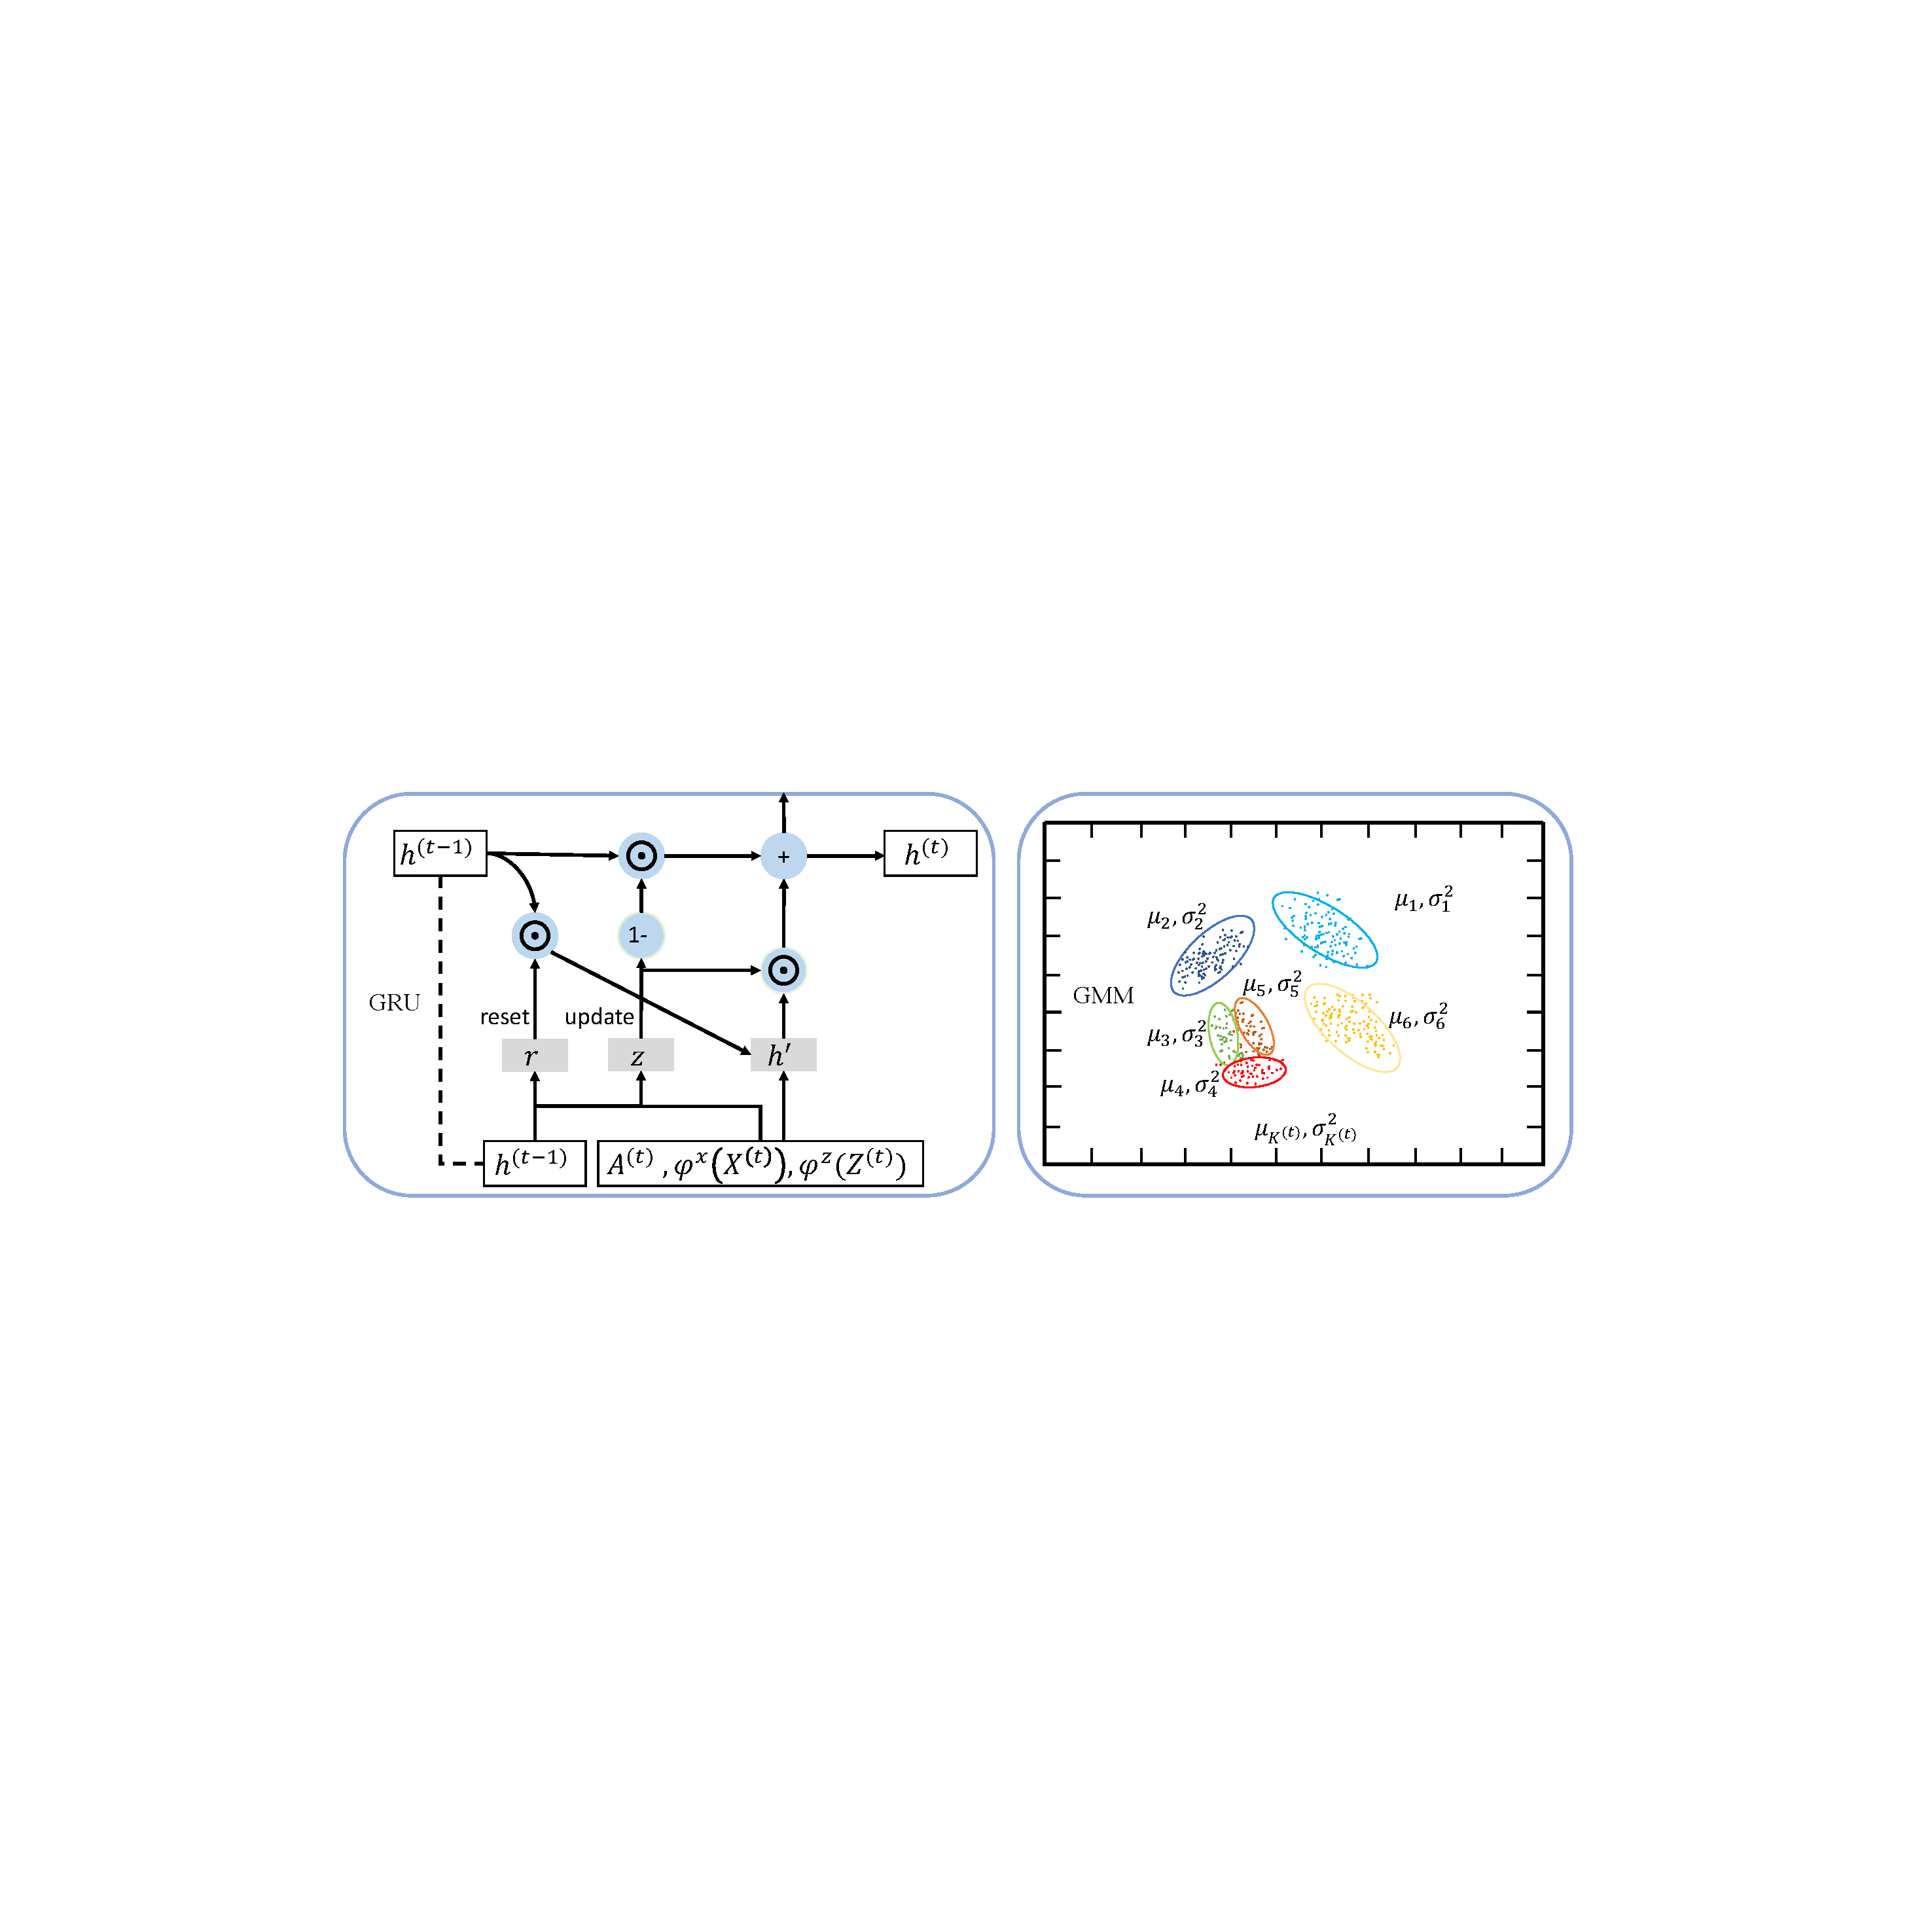
\includegraphics[width=.8\textwidth]{figures/chap06/GRU+GMM.pdf}
% \caption{Illustration of GRU and GMM in VGRGMM. The GRU unit takes $W^{(t)}$, $\varphi(X^{(t)})$ and $\varphi(Z^{(t)})$ as inputs, so that both graph topological dynamics and node attribute dynamics can be captured simultaneously. 
% The GMM modular replaces unimodal distribution with multimodal distribution at each snapshot, where $\bm{\mu}_{\bm{c}^{(t)}}$ and $\bm{\sigma}_{\bm{c}^{(t)}}^{2}$ ($\bm{c}^{(t)}\in [1, K^{t}]$) represent mean and variance of the $\bm{c}^{(t)}$-th community, respectively.} 
% \label{fig2}
% %\vspace{0cm}
% \end{figure*}

%============construct model===========
%===========Generation=================
\subsubsection{生成过程}


在$t$时刻,令节点$v_i$所属的社团$z_i^{(t)}$的概率分布定义如下:
\begin{equation}
z_i^{(t)} \sim \bm{Cat}(\bm{\pi}^{(t)}),
\label{eq:1}
\end{equation}
其中,$\bm{\pi}^{(t)}$是分类分布$\bm{Cat}(\bm{\pi}^{(t)})$的参数。$\bm{\pi}^{(t)} \in \boldsymbol{R}_{+}^{K^{(t)}}$的第$k$个分量,表示社团$z_k^{(t)}$的先验概率,且满足$\sum\nolimits_{k=1}^{K^{(t)}}{\pi_{k}^{(t)}}=1$。随后,对节点$v_i$生成一个基于其所属社团的潜在表示:
\begin{equation}
\mathbf{F}_i^{(t)} \Big| z_i^{(t)} \sim \bm{\mathcal{N}} \big(\bm{\theta}_{z_i^{(t)}}^{(t)}, (\bm{\sigma}_{z_i^{(t)}}^{(t)}\mathbf{I})^{2}\big),
\label{eq:2}
\end{equation}
其中,$\bm{\theta}_{z_i^{(t)}}^{(t)}$和$\bm{\sigma}_{z_i^{(t)}}^{(t)}$分别表示与社团$z_i^{(t)}$对应的高斯分布的均值和标准差,$\mathbf{I}$为单位矩阵。然后,对任意一对节点$(v_i,v_j)$,其在$t$时刻下的连边状态依据伯努利分布生成:
\begin{equation}
    \mathbf{W}^{(t)}_{i,j} \Big| \mathbf{F}^{(t)} \sim \bm{Bern}(b_{i,j}^{(t)}),
\label{chap6:eq:3}
\end{equation}
其中,$b_{i,j}^{(t)}$是关于$\mathbf{F}^{(t)}$的函数,可以是神经网络等高度灵活的函数形式。基于参考文献~\cite{kipf2016variational},本研究采用内积解码器来实现式~(\ref{chap6:eq:3}),具体如下:
\begin{align}
        p\big(\mathbf{W}^{(t)}_{i,j} =1 \,\big|\, \mathbf{F}_{i}^{(t)}, \mathbf{F}_{j}^{(t)}\big) 
        =  \sigma\Big(\mathbf{F}_{i}^{(t)}\big(\mathbf{F}_{j}^{(t)}\big)^{\top}\Big),
\label{eq:4}
\end{align}
其中,$\sigma(\cdot)$表示非线性函数,例如sigmoid。对$t$时刻全部节点对的联合概率可写为:
\begin{align}
        p(\mathbf{W}^{(t)} \big| \mathbf{F}^{(t)})  
        = \prod \limits_{i=1}^{N^{(t)}} \prod \limits_{j=1}^{N^{(t)}} p\big(\mathbf{W}_{i,j}^{(t)} \,\big|\, \mathbf{F}_{i}^{(t)}, \mathbf{F}_{j}^{(t)}\big).
\label{eq:5}
\end{align}

为表示社团成员关系,$t$时刻中定义了社团划分矩阵$\mathbf{Z}^{(t)} \in \{0,1\}^{N^{(t)}\times K^{(t)}}$,其中第 $i$ 行是一个one-hot向量,且 $\mathbf{Z}^{(t)}_{i,c_i^{(t)}} = 1$。基于上述整体生成过程,$\mathbf{W}^{(t)}$和$\mathbf{Z}^{(t)}$在给定$\mathbf{F}^{(t)}$的条件下相互独立。因此,可对所有时刻下的联合概率进行因式分解:
\begin{align}
    & p( \mathbf{W}^{(\leq T)},\mathbf{F}^{(\leq T)},  \mathbf{Z}^{(\leq T)}) \nonumber \\ 
    &=\prod_{t=1}^{T} p\bigl(\mathbf{W}^{(t)} \mid \mathbf{F}^{(t)}\bigr)\, p\bigl(\mathbf{F}^{(t)} \mid \mathbf{Z}^{(t)}\bigr)\, p\bigl(\mathbf{Z}^{(t)}\bigr)\label{eq:6}\\ \nonumber
    &=\prod_{t=1}^{T} \Bigl(\,\prod_{i=1}^{N^{(t)}} \prod_{j=1}^{N^{(t)}} p\bigl(\mathbf{W}_{i,j}^{(t)} \mid \mathbf{F}_{i}^{(t)}, \mathbf{F}_{j}^{(t)}\bigr)
    \prod_{i=1}^{N^{(t)}} p\bigl(\mathbf{F}_{i}^{(t)} \mid \mathbf{Z}_{i}^{(t)}\bigr)
    \prod_{i=1}^{N^{(t)}} p\bigl(\mathbf{Z}_{i}^{(t)}\bigr)\Bigr),
\end{align}
其中,$\mathbf{W}^{(\leq T)}$用于简化表示序列$\{\mathbf{W}^{(1)}, \mathbf{W}^{(2)}, \dots, \mathbf{W}^{(\leq T)} \}$,而$\mathbf{F}^{(\leq T)}$, $\mathbf{Z}^{(\leq T)}$以及后文的$\mathbf{X}^{(\leq T)}$也以同样方式简化表示。

上式中每个概率项的定义如下:
\begin{align}
    p\bigl(\mathbf{Z}_{i}^{(t)}\bigr)&=\bm{Cat}\bigl(c_i^{(t)} \mid \bm{\pi}^{(t)}\bigr), \label{eq:7}\\
    p\bigl(\mathbf{F}_{i}^{(t)} \mid \mathbf{Z}_{i}^{(t)}\bigr)&=\bm{\mathcal{N}}\Bigl(\bm{\theta}_{c_i^{(t)}}^{(t)}, \bigl(\bm{\sigma}_{c_i^{(t)}}^{(t)}\mathbf{I}\bigr)^{2}\Bigr), \label{eq:8}\\
    p\bigl(\mathbf{W}_{i,j}^{(t)} \mid \mathbf{F}_{i},\mathbf{F}_{j}\bigr)&=\bm{Bern}\bigl(b_{i,j}^{(t)}\bigr). \label{eq:91}
\end{align}

\subsubsection{推断过程}


本章在变分推理中采用证据下界(ELBO)来优化模型参数,并使用随机梯度变分推断(SGVI)进行训练。令$q(\mathbf{F}^{(t)}, \mathbf{Z}^{(t)})$ 为变分分布,用于近似后验分布 $p(\mathbf{F}^{(t)}, \mathbf{Z}^{(t)} \mid \mathbf{W}^{(\leq T)},\mathbf{X}^{(\leq T)})$。则可得到:
\begin{align}
\log p(\mathbf{W}^{(\leq T)},\mathbf{X}^{(\leq T)}) \ge \mathcal{L}\bigl(q,p\bigr) = \mathcal{E}[q(\mathbf{F}^{(\leq T)},\mathbf{Z}^{(\leq T)})] - \mathrm{KL}\bigl(q(\mathbf{F}^{(\leq T)},\mathbf{Z}^{(\leq T)})\parallel p(\mathbf{F}^{(\leq T)},\mathbf{Z}^{(\leq T)})\bigr),
\end{align}
其中$\mathrm{KL}(\cdot\parallel\cdot)$表示Kullback-Leibler散度。通过极大化该下界,可保证得到逼近真实后验的最优分布,从而学习到动态网络中社团划分与网络表示的有效参数。

%===============Inference===================


本研究使用变分后验分布$q(\cdot)$来逼近VGRGMM中的真实后验分布$p(\cdot)$。根据平均场假设,近似后验$q(\cdot)$不仅是$\mathbf{W}^{(t)}$和$\mathbf{F}^{(t)}$的函数,也与$\mathbf{h}^{(t-1)}$有关,因此可因式分解如下:
\begin{align}
        & q\bigl(\mathbf{F}^{(t)},\mathbf{Z}^{(t)}\mid \mathbf{W}^{(t)},\mathbf{X}^{(t)},\mathbf{h}^{(t-1)}\bigr) \nonumber\\
        & \qquad = q\bigl(\mathbf{F}^{(t)}\mid \mathbf{W}^{(t)},\mathbf{X}^{(t)},\mathbf{h}^{(t-1)}\bigr)\,q\bigl(\mathbf{Z}^{(t)}\mid\bm{W}^{(t)},\bm{X}^{(t)}\bigr). \label{eq:9}
\end{align}

\noindent 推断模型$q\bigl(\mathbf{F}^{(t)}\mid \mathbf{W}^{(t)},\mathbf{X}^{(t)},\mathbf{h}^{(t-1)}\bigr)$由一个两层GCN来参数化,其中第一层共享参数:
\begin{align}
    & q\bigl(\mathbf{F}_i^{(t)}\mid \mathbf{W}^{(t)},\mathbf{X}^{(t)},\mathbf{h}^{(t-1)}\bigr) 
    = \bm{\mathcal{N}}\bigl(\hat{\bm{\theta}}^{(t)}_i,\bigl(\hat{\bm{\sigma}}^{(t)}_i\mathbf{I}\bigr)^2\bigr), \nonumber\label{eq:10}\\
    & \hat{\bm{\theta}}^{(t)}=\mathrm{GCN}_{\hat{\bm{\theta}}}\Bigl(\mathbf{W}^{(t)}, \mathrm{GCN}_{s}\bigl(\mathbf{W}^{(t)},[\overline{ \Phi^{\mathbf{X}}\bigl(\mathbf{X}^{(t)}\bigr), \mathbf{h}^{(t-1)}} ]\bigr)\Bigr), \\
    & \log\hat{\bm{\sigma}}^{(t)}=\mathrm{GCN}_{\hat{\bm{\sigma}}}\Bigl(\mathbf{W}^{(t)}, \mathrm{GCN}_{s}\bigl(\mathbf{W}^{(t)},[\overline{ \Phi^{\mathbf{X}}\bigl(\mathbf{X}^{(t)}\bigr), \mathbf{h}^{(t-1)} }]\bigr)\Bigr), \nonumber
\end{align}
其中,$\hat{\bm{\theta}}^{(t)} \in \boldsymbol{R}^{N^{(t)}\times D}$与$\hat{\bm{\sigma}}^{(t)}\in \boldsymbol{R}^{N^{(t)}\times D}$分别表示近似后验分布的均值与标准差参数矩阵,其们的第$i$行分别对应$\hat{\bm{\theta}}^{(t)}_i$与$\hat{\bm{\sigma}}^{(t)}_i$。将$\mathbf{h}^{(t-1)}$复制$N^{(t)}$次以构造与$\Phi^{\mathbf{X}}(\mathbf{X}^{(t)})$相同行数的矩阵。此处采用了重参数化技巧:
\begin{equation}
    \mathbf{F}_{i}^{(t)} = \hat{\bm{\theta}}^{(t)}_i + \hat{\bm{\sigma}}^{(t)}_i \circ \bm{\epsilon}^{(t)},
    \label{eq:11}
\end{equation}
其中,$\bm{\epsilon}^{(t)}$表示辅助噪声变量,满足$\epsilon^{(t)} \sim \mathcal{N}(\bm{0}, \mathbf{I})$。

从文献~\cite{jiang2017variational}可得$q(\mathbf{C}^{(t)}\mid \mathbf{A}^{(t)},\mathbf{X}^{(t)})$的计算方式:
\begin{align}
    q\bigl(\mathbf{Z}_i^{(t)}\mid \mathbf{W}^{(t)},  \mathbf{X}^{(t)}\bigr)  &= p\bigl(z_i^{(t)}\mid \mathbf{F}^{(t)}_i\bigr) \nonumber \\ 
     &=  \frac{p\bigl(z_i^{(t)}\bigr)p\bigl(\mathbf{F}_i^{(t)}\mid z_i^{(t)}\bigr)}{\sum_{{z'}_i^{(t)}=1}^{K^{(t)}} p\bigl({z'}_i^{(t)}\bigr)p\bigl(\mathbf{F}_i^{(t)}\mid {z'}_i^{(t)}\bigr)}. \label{eq:12}
\end{align}


由式~(\ref{eq:9})可知,$q(\mathbf{F}^{(t)} \mid \mathbf{W}^{(t)},\mathbf{X}^{(t)},\mathbf{h}^{(t-1)})$与$\bm{h}^{(t-1)}$ 密切相关,其中$\bm{h}^{(t-1)}$由$\mathbf{W}^{(t-1)}$, $\mathbf{X}^{(t-1)}$ 以及$\mathbf{F}^{(t-1)}$推导得到。基于此,可进一步将$q\bigl(\mathbf{F}^{(\leq T)}, \mathbf{Z}^{(\leq T)} \mid \mathbf{W}^{(\leq T)}, \mathbf{X}^{(\leq T)}\bigr)$拆分如下:
\begin{align}
    q\bigl(\mathbf{F}^{(\leq T)}, & \mathbf{Z}^{(\leq T)} \mid \mathbf{W}^{(\leq T)}, \mathbf{X}^{(\leq T)}\bigr) \nonumber\\
    & = \prod_{t=1}^{T} q\bigl(\mathbf{F}^{(t)}, \mathbf{Z}^{(t)} \mid \mathbf{W}^{(\leq t)}, \mathbf{X}^{(\leq t)}, \mathbf{F}^{(< t)}\bigr), \nonumber\\
    & = \prod_{t=1}^{T} q\bigl(\mathbf{F}^{(t)}, \mathbf{Z}^{(t)} \mid \mathbf{W}^{(t)}, \mathbf{X}^{(t)}, \mathbf{h}^{(t-1)}\bigr).
    \label{eq:13}
\end{align}

为了便于表述,令$\Delta^{(\leq T)}$表示$ (\mathbf{F}^{(\leq T)}, \mathbf{Z}^{(\leq T)} \mid \mathbf{W}^{(\leq T)}, \mathbf{X}^{(\leq T)})$,令$\Delta^{(t)}$表示$(\mathbf{F}^{(t)}, \mathbf{Z}^{(t)} \mid \mathbf{W}^{(\leq t)}, \mathbf{X}^{(\leq t)}, \mathbf{F}^{(< t)})$。


%================Optimization=================
\subsection{优化过程}
%\subsubsection{Variational Lower Bound}
为了优化$q(\Delta^{(\le T)})$使其趋近于真实后验$p(\Delta^{(\le T)})$, 需要最小化KL散度$\mathbb{D_{\mathrm{KL}}}(q(\Delta^{(\le T)})||p(\Delta^{(\le T)}))$,其等价于最大化$p(\mathbf{W}^{(\leq T)},\mathbf{F}^{(\leq T)},\mathbf{Z}^{(\leq T)})$的$log$似然,亦称为变分下界(ELBO):
\begin{align}
\mathcal{L}_{ELBO} &= \log{p(\mathbf{W}^{(\leq T)}|\mathbf{F}^{(\leq T)},\mathbf{Z}^{(\leq T)})} \nonumber\\
& \quad \quad - \mathbb{D_{\mathrm{KL}}}(q(\Delta^{(\le T)})||p(\Delta^{(\le T)})) \nonumber\\
& = \mathbb{E}_{q(\Delta^{(\leq T)})}\Big[\log{p(\mathbf{W}^{(\leq T)}|\mathbf{F}^{(\leq T)},\mathbf{Z}^{(\leq T)})} \nonumber\\
& \quad \quad - \log{q(\Delta^{(\le T)})} + \log{p(\Delta^{(\le T)})}\Big] \nonumber \\
&= \mathbb{E}_{q(\Delta^{(\leq T)})} \Big[ \log{p(\mathbf{W}^{(\leq T)},\mathbf{F}^{(\leq T)},\mathbf{Z}^{(\leq T)})} \nonumber \\
& \quad \quad - \log{q(\Delta^{(\leq T)})} \Big]. \label{eq:14}
\end{align}


根据式~(\ref{eq:1}-\ref{chap6:eq:3})和式~(\ref{eq:10}),本研究通过使用SGVB~\cite{kingma2013auto}估计器,进一步具体化$\mathcal{L}_{ELBO}$为以下公式:
\begin{align} 
{\mathcal{L}_{ELBO}}  = &\sum_{t=1}^T \sum_{i=1}^{N^{(t)}}\Bigg[ \frac{1}{|\mathcal{S}_i^{(t)}|} \sum_{v_s\in \mathcal{S}_i^{(t)}} \Big[ \mathbf{W}_{i,s}^{(t)}\log{b_{i,s}^{(t)}} \nonumber\\
& + (1-\mathbf{W}_{i,s}^{(t)}) \log(1-\log{b_{i,s}^{(t)}}) \Big]\nonumber \\
&  + \sum_{z_i^{(t)}=1}^{K^{(t)}} \sum_{d=1}^{D}\Big[ \gamma_{z_i^{(t)}}^{(t)} \log\frac{\bm{\pi}_{z_i^{(t)}}^{(t)}}{\gamma_{z_i^{(t)}}^{(t)}} + \frac{1}{2} (1 + \log(\bm{\sigma}_{z_i^{(t)},d}^{(t)})^2) \nonumber\\
& - \frac{1}{2} \gamma_{z_i^{(t)}}^{(t)} \big[\log{(\bm{\sigma}_{z_i^{(t)},d}^{(t)})^2} + \frac{(\hat{\bm{\sigma}}_{i,d}^{(t)})^2}{(\bm{\sigma}_{z_i^{(t)},d}^{(t)})^2} \nonumber\\
& + \frac{({\hat{\bm{\theta}}}_{i,d}^{(t)} - \bm{\theta}_{z_i^{(t)},d})^{2}}{(\bm{\sigma}_{z_i^{(t)},d}^{(t)})^2}\big]\Big] \Bigg], 
\label{eq:16}
\end{align}

\noindent其中,$\mathcal{S}_i^{(t)}$是SGVB估计器中,$t$时刻节点$v_i \in V^{(t)}$的蒙特卡洛(MC)样本集,$\pi_{z_i^{(t)}}^{(t)}$表示社团$z_i^{(t)}$的先验概率,而$\gamma_{z_i^{(t)}}^{(t)}$表示$q(\mathbf{Z}_i^{(t)}|\mathbf{W}^{(t)},\mathbf{X}^{(t)})$。

\begin{algorithm}
	\caption{VGRGMM算法的伪代码} %
	%
	
	\algorithmicrequire ~迭代次数 $L$,邻接矩阵 $\mathbf{W}^{(\le T)}$ 和特征矩阵 $\mathbf{X}^{(\le T)}$。\\
	\algorithmicensure ~节点表示矩阵 $\mathbf{F}^{(\le T)}$ 和社团分配矩阵 $\mathbf{Z}^{(\le T)}$。 \\
	\begin{algorithmic}[1]
		\STATE {初始化:} $\bm{\pi^{(t)}} \sim \bm{\mathcal{U}(0,1)}$, 对于 $1 \le t \le T$;$ \mathbf{h}^{(0)}=\mathbf{0}$;
		\FOR {$t = 1,...,T$} \label{al:start}
		
		\STATE 根据式~(\ref{eq:10}) 获取高斯参数 $\hat{\mathbf{\theta}}^{(t)}$ 和 $\hat{\mathbf{\sigma}}^{(t)}$; \label{al:enstart} \\
		\STATE 根据式~(\ref{eq:11}) 生成节点表示矩阵 $\mathbf{F}_i^{(t)}$; \label{al:enend} \\
		\STATE 根据式~(\ref{eq:8}) 学习GRU隐藏状态 $\mathbf{h}^{(t)}$; \label{al:ev}
		\FOR {对于每个 $v_i \in V^{(t)}$}   \label{al:destart}
		\STATE 从分类分布 $\boldsymbol{Cat}(\bm{\pi}^{(t)})$ 中采样社团划分 $\mathbf{Z}_i^{(t)}$;
		\STATE 通过MC采样 $\mathcal{S}_i^{(t)} \subseteq V^{(t)}$~\cite{kingma2013auto};
		\FOR {对于每个 $v_s \in \mathcal{S}_i^{(t)}$}
		\STATE 根据式~(\ref{chap6:eq:3}) 重构邻接矩阵 $\mathbf{W}_{i,s}^{(t)}$;
		\ENDFOR
		\ENDFOR 
		\ENDFOR \label{al:deend}
		\STATE 根据式~(\ref{eq:16}) 计算 $\mathcal{L}_{ELBO}$; \label{al:trstart}
		\STATE 通过随机梯度下降最大化 $\mathcal{L}_{ELBO}$ 并更新 VGRGMM 中的参数。\label{al:end} \label{al:trend}
		\STATE \textbf{重复} 第 \ref{al:start}-\ref{al:end} 行,直到达到迭代次数限制 $L$。
		\STATE 根据式~(\ref{eq:12}) 获取社团分配矩阵 $\mathbf{Z}^{(\le T)}$。 \label{al:ass}
		\RETURN $\mathbf{F}^{(\le T)}$ 和 $\mathbf{Z}^{(\le T)}$
		
	\end{algorithmic}
	\label{algorithm:chap6}
\end{algorithm}

本研究接下来将探讨如何通过最大化$\mathcal{L}_{ELBO}$来对模型进行求解:
\begin{align}
 {\mathcal{L}_{ELBO}} & = \sum_{t=1}^T \int_{\bm{F}^{(t)}} \sum_{z_i^{(t)}} q(\bm{F}^{(t)}|\bm{W}^{(t)},\bm{X}^{(t)},\bm{F}^{(<t)})q(z_i^{(t)}|\bm{W}^{(t)},\bm{X}^{(t)}) \nonumber \\
 & \quad \cdot\log\Bigg[\frac{p(\bm{X}^{(t)}, \bm{W}^{(t)} | \bm{F}^{(t)}) p(\bm{F}^{(t)})}{q(\bm{F}^{(t)}|\bm{X}^{(t)},\bm{W}^{(t)}, \bm{F}^{(< t)})} \cdot\frac{p(z_i^{(t)}|\bm{F}^{(t)})}{q(z_i^{(t)}|\bm{X}^{(t)},\bm{W}^{(t)})} \Bigg]d\bm{F}\nonumber\\
 & = \sum_{t=1}^T \Bigg[\int_{\bm{F}^{(t)}}q(\bm{F}^{(t)}|\bm{W}^{(t)},\bm{X}^{(t)},\bm{F}^{(< t)}) \nonumber \\ 
 & \quad \quad \quad \cdot \log\frac{p(\bm{X}^{(t)}, \bm{W}^{(t)} | \bm{F}^{(t)}) p(\bm{F}^{(t)})}{q(\bm{F}^{(t)}|\bm{X}^{(t)},\bm{W}^{(t)}, \bm{F}^{(< t)})} d\bm{F} \nonumber \\
 & \quad - \int_{\bm{F}^{(t)}} q(\bm{F}^{(t)}|\bm{W}^{(t)},\bm{X}^{(t)},\bm{F}^{(< t)}) \nonumber\\
 & \quad \quad \cdot D_{KL}\left[q(z_i^{(t)}|\bm{X}^{(t)},\bm{W}^{(t)}) \parallel p(z_i^{(t)}|\bm{F}^{(t)})\right] d\bm{F} \Bigg],
\end{align}
其中,前项与社团$z$无关,后项为$KL(\cdot || \cdot)$散度,显然是非负的。因此,当$\mathcal{L}_{ELBO}$达到最大值时,$D_{KL}\left[q(z_i^{(t)}|\bm{X}^{(t)},\bm{W}^{(t)}) \parallel p(z_i^{(t)}|\bm{F}^{(t)})\right] dF =0$是最适合的。 
% \fi
% \iffalse
因此,在式~(\ref{eq:14})中计算$q(z_i^{(t)}|\bm{W}^{(t)},\bm{X}^{(t)})$遵循以下等式:
\begin{equation}
    q(z_i^{(t)}|\bm{W}^{(t)},\bm{X}^{(t)}) = p(z_i^{(t)}|\bm{F}^{(t)}) =\frac{p(z^{(t)})p(\bm{F}^{(t)}|z_i^{(t)})}{\sum_{z^{'}=1}^{K^{(t)}} p(z^{'})p(\bm{F}^{(t)}|z^{'})}.
\end{equation}

由于$Z^{(t)}$与$\bm{F}^{(t)}$存在较强的相关性,因此可以减少均场假设导致的信息丢失。



%\begin{algorithm}
%	\caption{VGRGMM算法的伪代码}
%	\algorithmicrequire ~迭代次数 $L$,邻接矩阵 $\mathbf{W}^{(\le T)}$,特征矩阵 $\mathbf{X}^{(\le T)}$ \\
%	\algorithmicensure ~节点表示矩阵 $\mathbf{F}^{(\le T)}$,社团分配矩阵 $\mathbf{Z}^{(\le T)}$ 
%	\begin{algorithmic}[1]
%		\STATE 初始化:$\bm{\pi^{(t)}} \sim \bm{\mathcal{U}(0,1)}$ ($1 \le t \le T$),$\mathbf{h}^{(0)}=\mathbf{0}$
%		\FOR {$t = 1,...,T$} 
%		\STATE 获取高斯参数 $\hat{\mathbf{\theta}}^{(t)}, \hat{\mathbf{\sigma}}^{(t)}$ (式~(\ref{eq:10}))
%		\STATE 生成节点表示 $\mathbf{F}_i^{(t)}$ (式~(\ref{eq:11}))
%		\STATE 学习GRU隐藏状态 $\mathbf{h}^{(t)}$ (式~(\ref{eq:8}))
%		\FOR {每个 $v_i \in V^{(t)}$}
%		\STATE 采样社团划分 $\mathbf{Z}_i^{(t)} \sim \boldsymbol{Cat}(\bm{\pi}^{(t)})$
%		\STATE MC采样 $\mathcal{S}_i^{(t)} \subseteq V^{(t)}$~\cite{kingma2013auto}
%		\STATE 重构 $\mathbf{W}_{i,s}^{(t)}$ ($v_s \in \mathcal{S}_i^{(t)}$, 式~(\ref{chap6:eq:3}))
%		\ENDFOR
%		\ENDFOR
%		\STATE 计算 $\mathcal{L}_{ELBO}$ (式~(\ref{eq:16}))
%		\STATE 通过SGD最大化 $\mathcal{L}_{ELBO}$ 更新参数
%		\STATE 重复步骤 2-10 直到迭代 $L$ 次
%		\STATE 获取社团分配 $\mathbf{Z}^{(\le T)}$ (式~(\ref{eq:12}))
%		\RETURN $\mathbf{F}^{(\le T)}, \mathbf{Z}^{(\le T)}$
%	\end{algorithmic}
%	\label{algorithm:chap6}
%\end{algorithm}
算法~\ref{algorithm:chap6}提供了VGRGMM方法的伪代码。其中\ref{al:enstart}-\ref{al:enend}行对应编码(推断)过程,而~\ref{al:destart}-\ref{al:deend}行对应解码(生成)过程。~\ref{al:ev}行是捕捉演化依赖性的过程。~\ref{al:trstart}行和~\ref{al:trend}行描述了每次训练迭代的优化过程。VGRGMM与其他基于网络表示学习的动态社团检测方法的最大区别在于,一旦VGRGMM训练完成,其可以自然地为所有快照中的节点分配社团,如~\ref{al:ass}行所示。
% 其中选择概率最大的社团。




VGRGMM的复杂度为$O(TND^2W)$,其中,$W$是GRU的所有参数数量,其复杂度与大部分同类方法相差不大,且依赖于对社团初始化的效果,可以通过对每个快照进行谱聚类以提升其计算效率。

\section{VGRGMM模型实验\label{chap6:experiment}}

本节将引入多种动态网络数据集和对比方法,并在社团检测任务上使用了四种评估指标来验证VGRGMM方法在社团检测任务中的效果。

\subsection{数据集}
本节选择了三类动态网络数据集,包括$12$个动态网络数据:
\begin{itemize}
    \item \textbf{生成数据集}:此类数据包含两组数据集,第一个生成数据集是根据~\cite{kim2009particle}和~\cite{Lin.2009.Tseng}进行生成的,该数据是一个具有数量可变的社团真相的动态网络数据集。在第一个快照中,网络结构基于随机块模型生成,随后在每个快照$t \ge 2$时,改变社团结构并利用~\cite{Lin.2009.Tseng}公布的参数来设置动态网络的演化。另一个生成数据集来自~\cite{ditursi2017local},其可以生成具有幂律分布的动态网络,网络结构的变化由不同社团中的节点转移进行驱动。本文称这两个动态网络为Var和Synth,其统计数据见表~\ref{tab1},其他参数设置可在~\cite{kim2009particle}和~\cite{Lin.2009.Tseng}中找到。上述两个生成数据均具有社团真相。
    \item \textbf{具有真实社团标签的真实社交网络}:包含四个动态社交网络,即 HS11~\cite{stehle2011high}、HS12~\cite{stehle2011high}、Primary~\cite{stehle2011high} 和 Workplace~\cite{genois2014data}。这些网络中的节点代表人,边表示人和人之间的通信关系,社团表示社交圈、兴趣组或班级。
    \item \textbf{无真实标签的真实网络}:包含 Cellphone~\cite{folino2013evolutionary}(电信网络)、Enron\footnote{http://www.cs.cmu.edu/~enron}(电子邮件网络)、Voles~\cite{rossi2015network}(动物交互网络)、Fbmessages~\cite{rossi2015network}(加州大学的社交网络)以及两个更大规模的网络 iadublin\footnote{http://www.sociopatterns.org/datasets/} 和 soc-wiki~\cite{rossi2015network}用以验证各模型在较大规模网络中的运行效率。
\end{itemize}

\begin{table}[htbp]
	\caption{动态网络的统计数据}\label{tab1}
	\vspace{0.5em}\centering\wuhao
	\centering%居中
	\renewcommand\arraystretch{1}{
		\begin{tabular}{ccccccc}
			\toprule
			\centering
			~~数据集~~ & ~ $T$~ &~  $\overline{N}$ ~& ~$\overline{M}$~ & ~$\overline{K}$~ & ~$\overline{d_{\mathrm{avg}}}$~ & ~$\overline{\mathrm{cc}_{\mathrm{avg}}}$~\\
			\hline
			Var &  10 & 393 & 3,055 & 8 & 15.4926 & 0.1622\\ 
			
			Synth &  10 & 15,000 & 300,000 & 8 & 20.000 & 0.2530\\ 
			
			HS11 &  7 & 126 & 424 & 5 & 6.7336 & 0.2611\\
			
			HS12 &  8 & 180 & 538 & 7 & 5.9778 & 0.2599\\
			
			Primary &  6 & 242 & 2,977 & 13 & 24.6102 & 0.5269\\
			
			Workplace &  8 & 92 & 175 & 6 & 3.8207 & 0.2152\\
			
			Cellphone &  10 & 400 & 512 & - & 2.5620 & 0.0141\\
			
			Enron &  12 & 151 & 292 & - & 4.0138 & 0.4075\\
			
			Voles &  7 & 1,686 & 4,739 & - & 0.8041 & 0.0768\\
			
			fbmessages &  6 & 1,899 & 15,648 & - & 2.9137 & 0.1551\\
			
			iadublin & 8 & 10,972 & 415,913 & - & 75 & 1.0607\\
			
			soc-wiki & 12 & 7,118 & 100,811 & - & 28.3257 & 0.1408 \\
			\bottomrule
	\end{tabular}} 
	\vspace{0cm}
\end{table}


上述动态网络的统计数据汇总如表~\ref{tab1}所示。$\overline{N}$、$\overline{M}$、$\overline{K}$、$\overline{d_{\mathrm{avg}}}$ 和 $\overline{\mathrm{cc}_{\mathrm{avg}}}$ 分别表示所有快照中节点、边、社团的平均数量,平均度和平均聚类系数。







\subsection{实验设置}

为了进行全面的比较,本节将VGRGMM与动态网络中流行的社团检测方法进行了比较,包括非深度学习方法DYNMOGA~\cite{folino2013evolutionary}和DECS~\cite{liu2020detecting},以及基于深度学习的动态网络表示学习方法,包括DynGEM~\cite{goyal2018dyngem}、AdaDyGNN~\cite{Li2024DyGNN}、CDNMF~\cite{li2024contrastive}、DynRNN~\cite{goyal2020dyngraph2vec}、DynAERNN~\cite{goyal2020dyngraph2vec}和VGRNN~\cite{hajiramezanali2019variational}。其中动态网络表示学习方法在获得节点的时序表示向量后,通过混合高斯聚类识别网络中的社团结构。各方法的技术路线总结如下:
%选择了七种先前发表的代表性方法,根据非深度学习模型(AFFECT、DYNMOGA和DECS)和深度学习模型(DynGEM、DynAE、DynRNN、DynAERNN和VGRNN)的分类来检测社团,其中动态网络嵌入通过GMM方法获得并用于聚类。
\begin{itemize}
%    \item \textbf{AdaDyGNN}~\cite{Li2024DyGNN}:该方法属于经典的进化聚类算法,不同于大部分进化聚类算法将时间平滑性融入到损失函数中,该方法通过精确追踪社团随时间变化的临近性来实现对动态社团演化的建模。
 	\item \textbf{AdaDyGNN}~\cite{Li2024DyGNN}:该方法从动态网络演化过程中节点与边的噪声过滤角度设计了基于强化学习的动态图神经网络知识自适应框架,通过将节点变化的选择问题转化为序列决策过程实现对动态网络的鲁棒性表示学习。
    \item \textbf{DYNMOGA}~\cite{folino2013evolutionary}:该方法将动态网络中的社团检测任务视为一个多目标优化问题。第一个目标是在当前快照搜索社团结构,第二个目标则是最小化当前快照与前一个快照的社团结构差异以捕获时序平滑性。
    \item \textbf{DECS}~\cite{liu2020detecting}:该方法在经典进化聚类算法的基础上,提出了新的基因突变算子来确保节点及其邻居有更大的概率划分到同意社团,并引入了基因矩阵来编码网络结构信息以提升社团搜索效率。
    \item \textbf{DynGEM}~\cite{goyal2018dyngem}:该方法以深度自编码器为核心,利用深度学习生成高度非线性的节点表示并以此重构所观测到的动态网络。
%    \item \textbf{DynAE}~\cite{mrabah2019deep}:该方法将节点聚类引入动态自编码器的目标函数,并提出在训练过程逐步调整权重以平衡网络重构与节点聚类两个目标函数的比重来提升网络表示学习在节点聚类任务的效果。
	\item \textbf{CDNMF}~\cite{li2024contrastive}:基于深度非负矩阵分解的静态社团检测算法,该方法通过深度神经网络提升模型的信息抽取能力,并构建了网络拓扑与节点属性的对比学习机制以提升模型的社团检测效果。
    \item \textbf{DynRNN}~\cite{goyal2020dyngraph2vec}:该方法以当前时刻之前的所有网络快照作为输入,利用RNN建模网络的时序演化模式,将当前时刻的网络结构作为输出,从而能够捕捉每个快照节点之间以及多个快照的非线性交互。
    \item \textbf{DynAERNN}~\cite{goyal2020dyngraph2vec}:该方法的模型框架与DynRNN相同,改进点主要关注对动态网络快照的重构,通过自编码器来对其进行实现。
    \item \textbf{VGRNN}~\cite{hajiramezanali2019variational}:该方法在时序建模中依然通过RNN来实现,但其自编码器部分为节点引入了先验概率(即变分自编码器),并利用变分推断与SGVB实现对随机变量的梯度传播。
    \item \textbf{VGAECD}:该方法在静态网络上独立使用变分图自编码器进行社团检测。其思路与\cite{choong2018learning}中的方法一致,也是本章所提出VGRGMM方法中忽略动态网络快照间依赖关系的特例,可以视作消融。
\end{itemize}


对于非深度学习模型,其参数基于原始论文中的设置,以保证最佳性能。而对于深度学习模型,本章对这些模型的参数进行了微调,以在不同数据集上获得最佳性能。对于本研究的模型,在所有数据集中设置了一个包含$32$个GRU单元的单一循环隐藏层。在编码过程中,使用了一个大小为 $[32,16]$的两层GCN来推导$\hat{\bm{\theta}}^{(t)}$和$\hat{\bm{\sigma}}^{(t)}$,并为$\Phi^{\mathbf{X}}$和$\Phi^{\mathbf{F}}$设置了两个$32$维的全连接层。此外,本研究进行了$L=1,000$次迭代训练,学习率为$0.01$,或直到模型收敛。

由于大多数方法都预先设置了动态网络的社团数量$K^{(1)}, K^{(2)}, \cdots, K^{(T)}$,本研究将其设置为真实的社团数量。对于没有社团真相的动态网络,本研究使用当前常用的方法~\cite{Krzakala.2013.Zhang}在每个快照上计算社团个数。超参数 $K^{(1)},K^{(2)},\cdots,K^{(T)}$首先设置为一个足够大的数值(如$log(N)$),然后VGRGMM通过舍弃冗余社团来获得实际的社团数量。


\subsection{评价指标}
本章引入四种广泛使用的指标来评估社团检测的性能,具体如下。
\begin{itemize}
  \item \textbf{归一化互信息(NMI)}:其衡量了在$t$时刻,计算得到的社团划分$\mathcal{C}^{(t)}$ 与真实社团划分$\mathcal{C}_{\mathrm{T}}^{(t)}$之间的相似程度。NMI值越高,社团检测效果越好。
\item \textbf{精度(AC)}~\cite{folino2013evolutionary}:其通过与真实值的比较来衡量社团划分效果。AC值越低,社团检测性能越好。

\item \textbf{调整兰德指数(ARI)}:其是一个数据聚类指标,用于衡量模型计算的社团划分$\mathcal{C}^{(t)}$与真实社团划分$\mathcal{C}_{\mathrm{T}}^{(t)}$之间的相似性。ARI越高表示社团检测效果越好。

\item \textbf{模块度(Q)}:其衡量了所划分社团内节点连边的紧密程度,其通过对比所识别社团结构在网络快照中的紧密程度与空模型的紧密程度之差。模块度越高,表示社团内节点连边越紧密,社团间节点连边越稀疏。
\end{itemize}
需要注意的是,\emph{NMI}、\emph{AC}和\emph{ARI}仅在数据中存在社团标签时适用,而$Q$可以在没有真实社团标签的情况下进行测量。较大的\emph{NMI}、\emph{ARI}和$Q$值表示社团划分结果更好,而\emph{AC}越小则表示社团划分结果更好。
各评价指标的详细定义见~\ref{chap2:metrics}




%======================Experiment Results===========================
\subsection{动态社团检测实验结果}



为了评估VGRGMM在动态社团检测中的效果,本节将其与对比方法在流行的生成和真实动态网络上进行了比较。对于具有真实标签的动态网络,结果基于\emph{NMI}、\emph{AC}和\emph{ARI}进行评估。对于没有标签的数据集,本研究使用模块度$Q$来评估不同方法的效果。



\subsubsection{生成数据集实验结果}

\begin{figure*}[htbp]
    \centering
    \hspace{-2mm}
    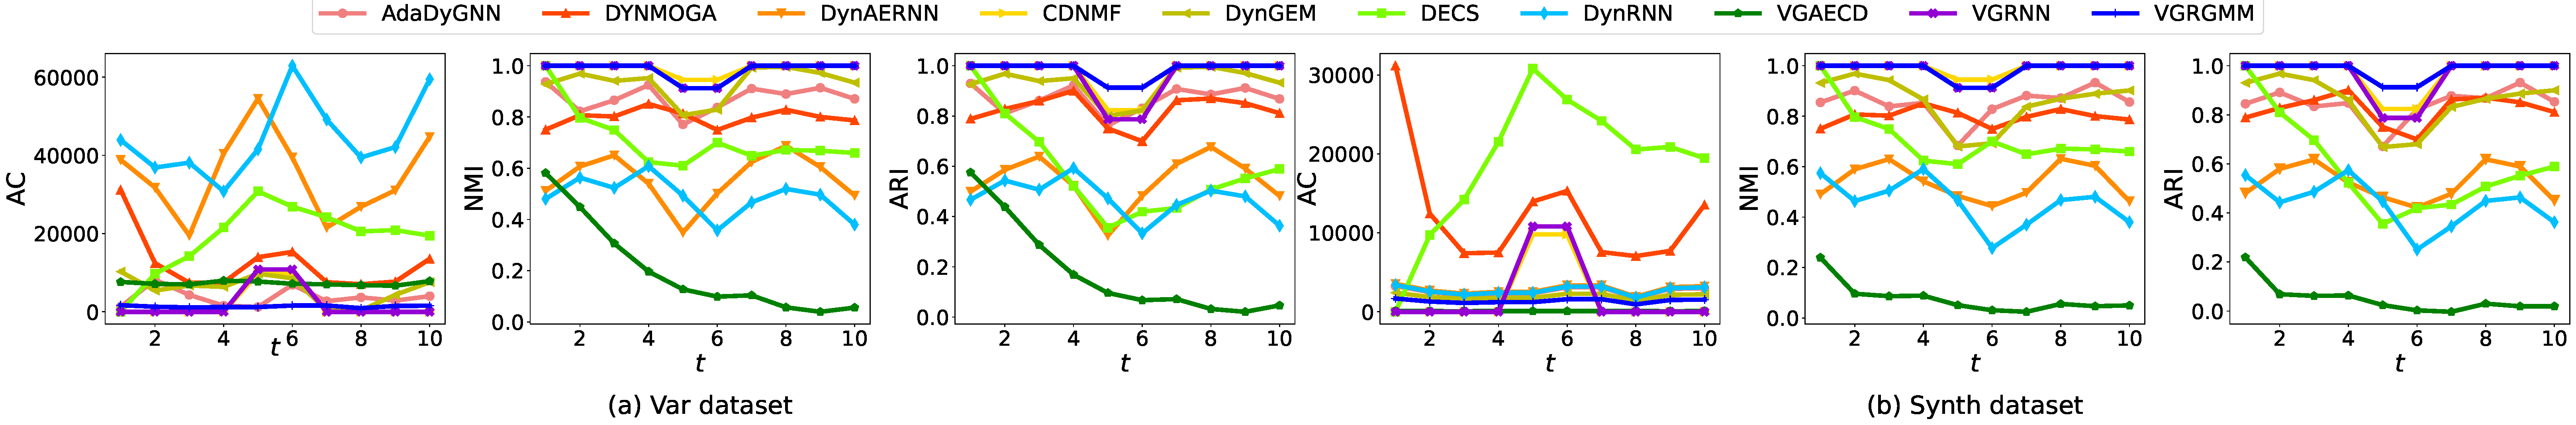
\includegraphics[width=1\textwidth]{figures/chap06/chap5synthData.pdf}
    \caption{两种生成的动态网络的实验结果对比。(a) Var 数据集, (b) Synth 数据集。图中每个值是基于$10$次具有相同参数的随机生成网络的计算的平均值。}
    \label{fig:gene}
\end{figure*}

如图~\ref{fig:gene}所示,本节展示了所有方法在生成的数据集Var和Synth(网络规模更大)上的社团检测结果。在\emph{NMI}、\emph{AC}和\emph{ARI}指标上对这些方法进行了评估。

对于两种不同规模的网络,本节的方法VGRGMM在所有三个指标上几乎表现最佳。CDNMF和VGRNN相较于VGRGMM具有一定竞争力,并且优于其他对比方法。CDNMF的对比学习机制能够有效地捕获网络的全局特征,VGRNN则捕捉了动态网络的时序演化以及高维和非线性结构。另一方面,深度表示学习方法DynRNN和DynAERNN仅专注于建模网络拓扑的动态变化,因此未能捕捉到动态社团的结构信息。经典的动态社团检测方法DYNMOGA通过多目标函数优化获得社团结构,也取得了较好的表现。此外,静态方法VGAECD在所有数据集和指标上表现非常差,因其无法建模网络与社团的演化。总体而言,VGRGMM能够有效建模跨快照建模时序依赖性,并使用GMM先验捕获了社团结构信息,并建模了动态网络的非线性结构,因此能在节点和社团层面的任务获得更好的表现。



\subsubsection{真实世界网络的实验结果}


\begin{figure*}[htbp]
    \centering

    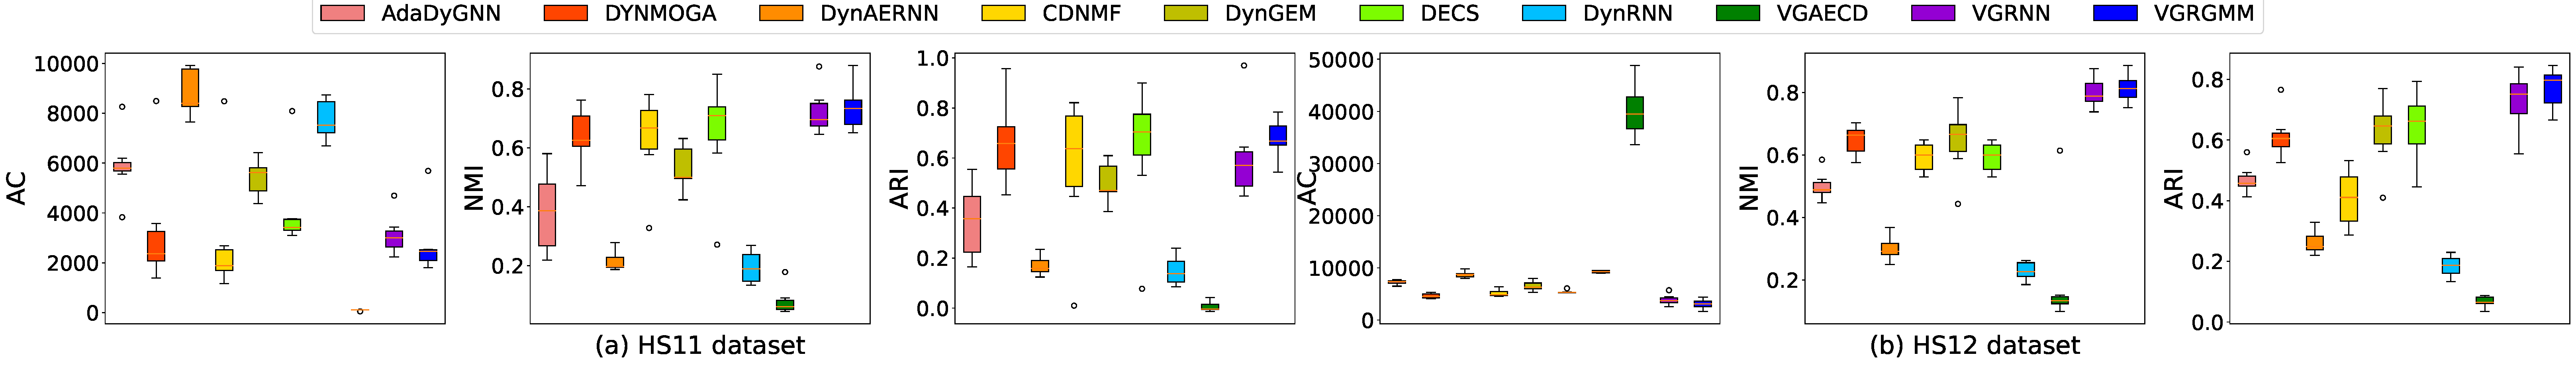
\includegraphics[width=1\textwidth]{figures/chap06/chap5realDataGHS-box.pdf}
    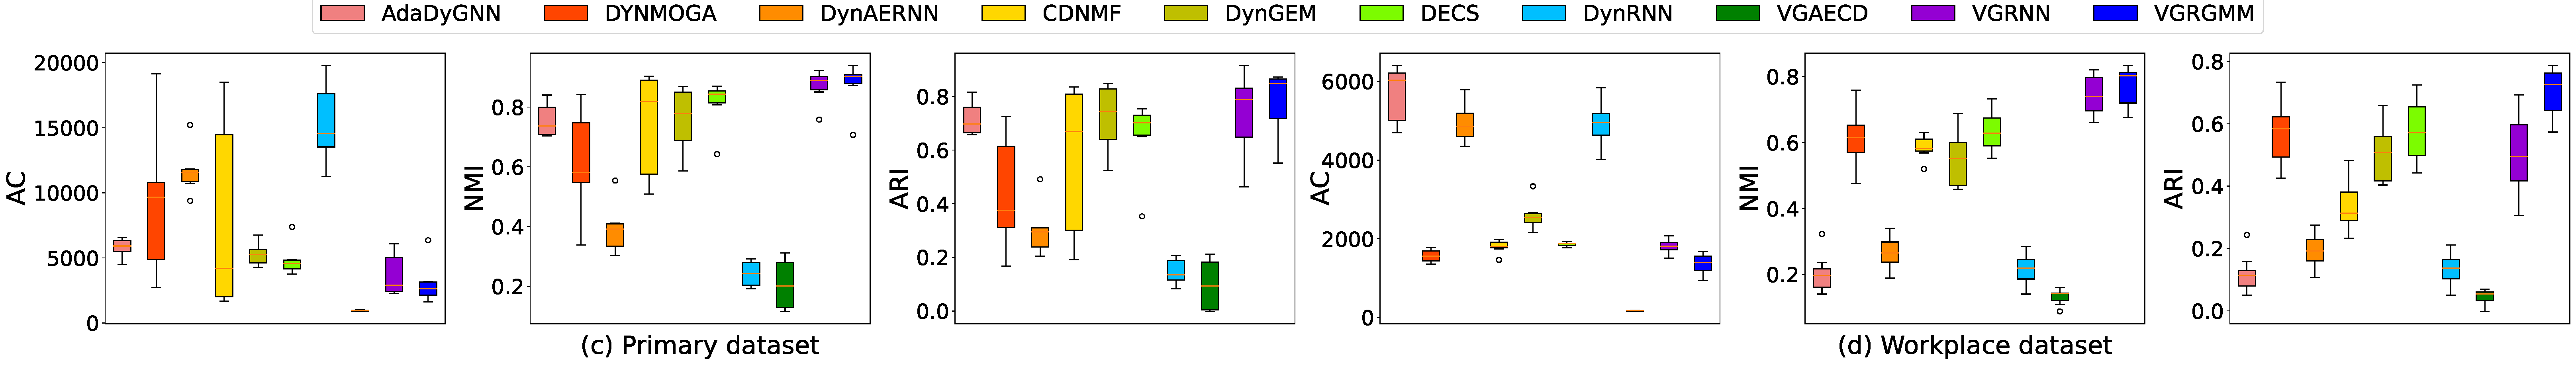
\includegraphics[width=1\textwidth]{figures/chap06/chap5realDataGpw-box.pdf}
    \caption{四个具有真相的真实世界动态网络的社团检测结果}
    \label{fig:realnet}
    \vspace{0cm}
\end{figure*}

\begin{figure*}[htbp]
    \centering
    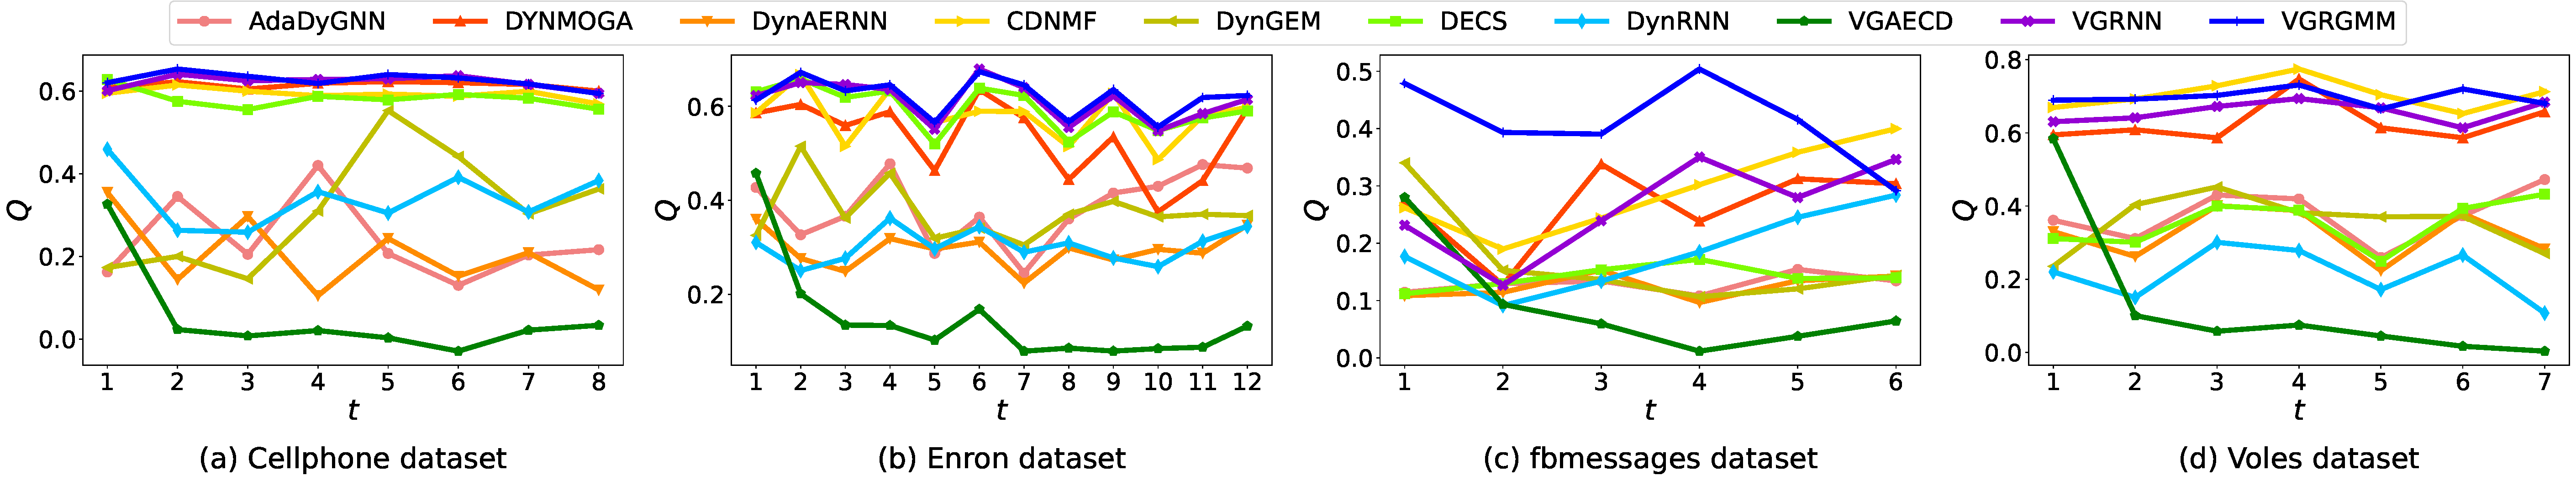
\includegraphics[width=1\textwidth]{figures/chap06/chap5realDataNG.pdf}
    \caption{在没有真实标签的真实世界数据集上的社团检测结果}
    \label{fig:noTruth}
    \vspace{0cm}
\end{figure*}

本节展示了在真实世界数据集上的实验结果,这些数据集分为有真实标签和无真实标签的动态网络。图~\ref{fig:realnet}展示了不同方法在四个具有社团真相的动态网络上的结果,使用\emph{NMI}、\emph{AC}和\emph{ARI}指标进行评估。为了使比较更加清晰,本章使用箱形图展示了所有方法在每个动态网络上的社团检测效果,每个箱形图表示$30$次实验结果的平均值和标准差。总体而言,本研究的VGRGMM在这三个指标上的表现均优于其他对比方法,较小的标准差意味着其在快照间具有稳定和平滑的结果。VGAECD表现较差,因为其仅忽略了动态网络的时序演化,这意味着动态网络的历史信息对于动态社团检测非常重要。对于其他对比方法,没有一个方法在所有网络上都能与本研究的方法竞争。尽管VGRNN在整体上表现第二好,但在HS11数据集上不如DECS。

本章还展示了对于没有社团真相的动态网络的实验结果,基于模块度$Q$进行评估,如图~\ref{fig:noTruth}所示,VGRGMM在图中的四组网络上也表现出最佳或次佳的性能。此外,VGRGMM、DYNMOGA、DECS和VGRNN都表现出优异的结果,因为这些方法要么模型设计是基于模块度优化进行的改进,要么建模了动态网络的时序演化。

\begin{table}
\centering
% \begin{table*}
\caption{\label{tab2}不同方法的运行时间对比(s)}
\vspace{0.5em}\centering\wuhao
 \begin{tabular}{cp{0.7cm}p{0.7cm}p{0.7cm}p{0.7cm}p{0.7cm}p{0.7cm}p{0.7cm}p{0.85cm}p{0.85cm}p{0.7cm}}
\hline
\diagbox{方法名}{数据集}& Var & HS11 & HS12 & Pri & Work & Cphone & Enron & Voles & fbmsg & Synth \\
\hline
AdaDyGNN & 91.7 & 57.5 & 65.9 & 75.1 & 52.3 & 91.1 & 60.6 & 382.2  & 254.8 & 10943.2\\

DynAERNN & 94.9 & 75.1 & 70.7 & 76.9 & 61.8 & 96.4 & 78.1 & 388.1 & 289.8 & 10102.3\\

DynRNN & 103.5 & 83.2 & 77.1 & 78.2 & 66.2 &103.3 & 81.4 &271.8 & 299.0 & 9862.5\\

DynGEM & 47.0 & 4.5 & 5.8 & 40.9 & 2.2  & 7.4 &   3.5 & 19.0 & 87.8 & 5620.1 \\

DYNMOGA & 2601.2& 1937.5 & 2017.0 & 1903.9 & 2532.8 & 3012.1 & 2109.4 & 8904.7 & 8936.9 & 35724.6\\

DECS & 2930.1 & 2632.1 & 2500.2 & 2610.8 & 2712.0 & 2812.9 &  2633.0 & 10389.7 & 11397.4 & 33761.9\\

CDNMF & 2814.6 & 2477.8 & 2530.2 & 2634.3 & 2262.4 &2822.9 & 2494.7 & 11111.8 & 12532.6 & 38650.2\\

VGRNN+GMM & 100.8 & 106.5 & 21.9 & 51.4 & 114.8 & 37.4 &  17.2 & 96.5 & 127.9 & 9620.4\\

VGRGMM & 35.4 & 5.522 & 8.9 & 22.8 & 6.4& 32.9 &  12.2 & 12.7 & 40.0 & 9036.1\\
\hline
\end{tabular} 

% \end{table*}
\end{table}


\subsubsection{大规模数据实验结果}
为验证所提出的VGRGMM的计算效率,本节将社团检测效果较好的对比方法的运行时间成本与VGRGMM进行了对比。所有方法均在相同的实验环境中运行(使用CPU),并将训练轮数(epoch)设置为$50$,并计算其运行时间的平均值,结果如表~\ref{tab2}所示,其中Pri表示Primary数据集、Work表示Workplace数据集、Cphone表示CellPhone数据集、fbmsg表示fbmessages数据集。
% %Result is shown in Table~\ref{tab2}.
\begin{figure}
    \centering
    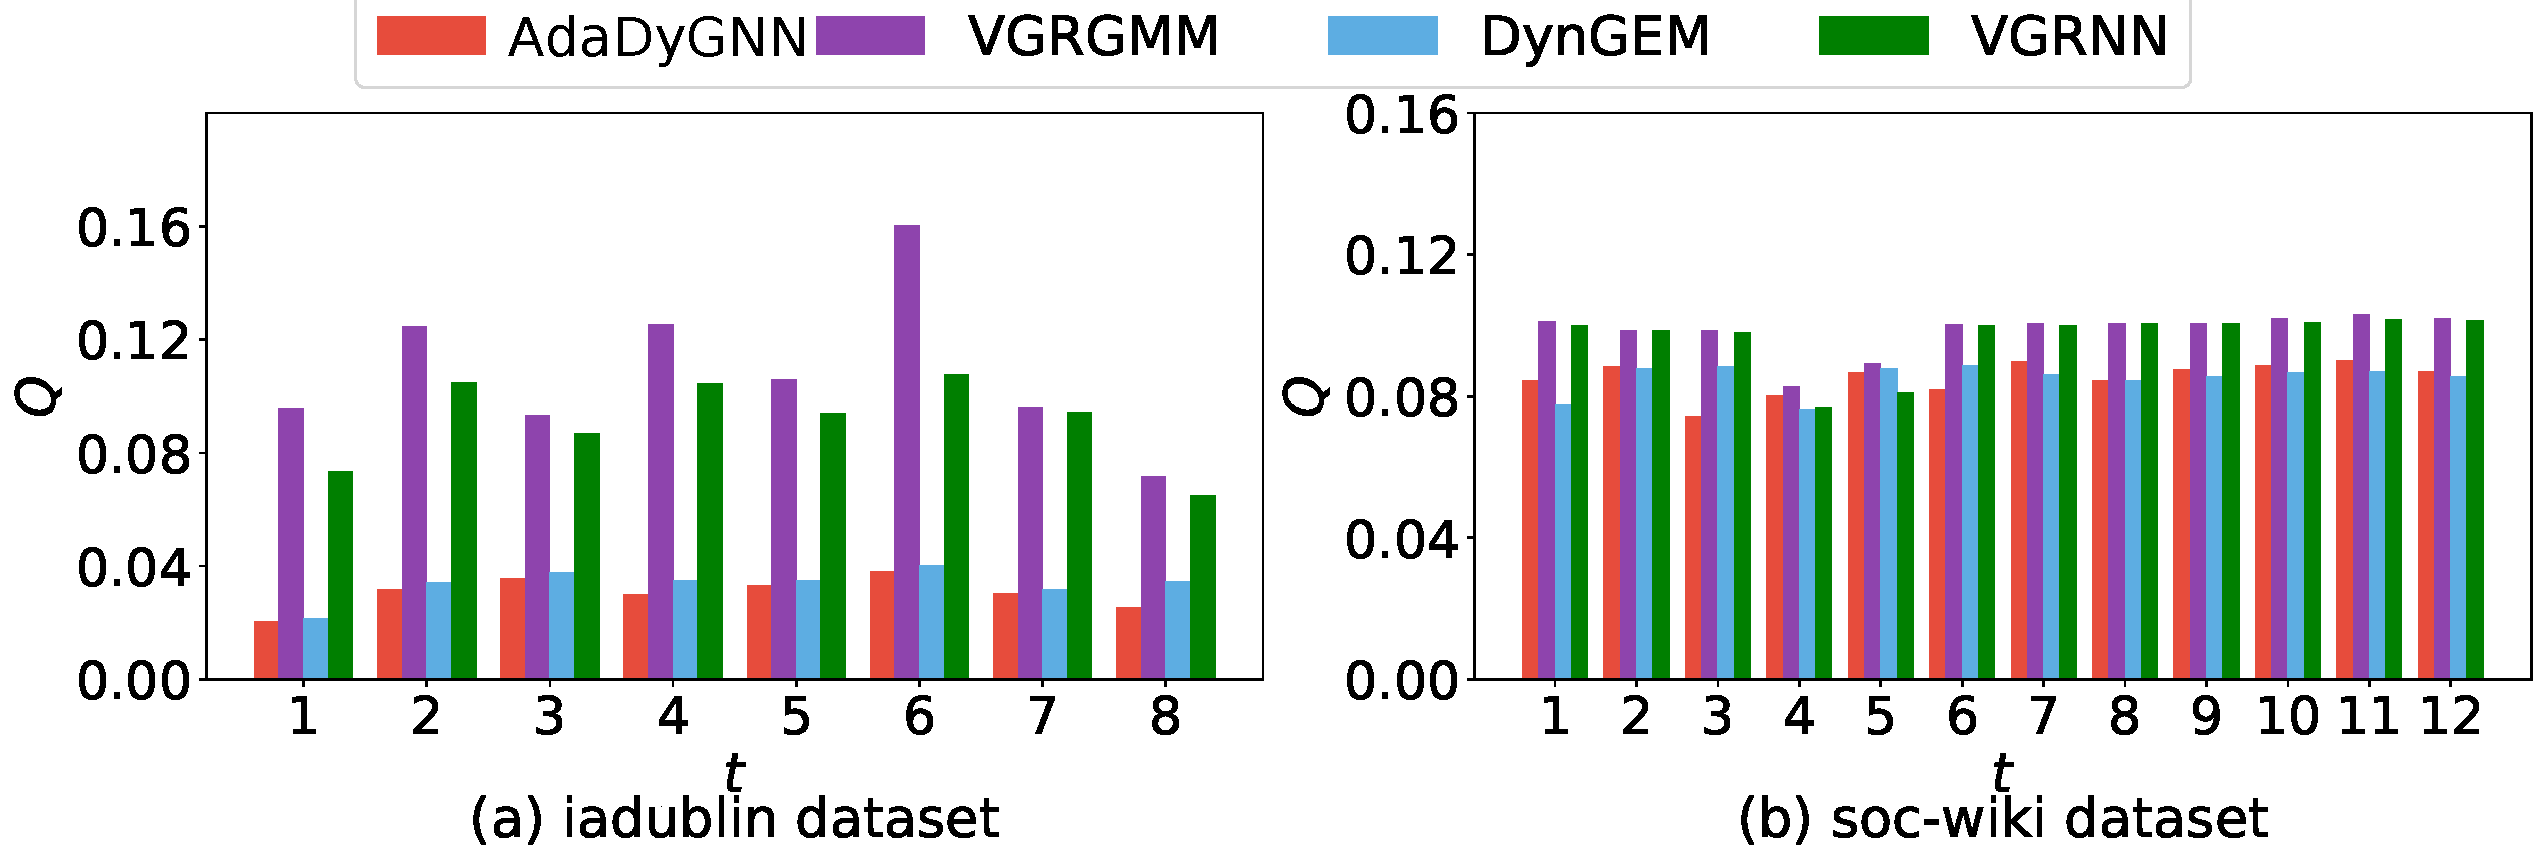
\includegraphics[width=.8\textwidth]{figures/chap06/chap5bigdata-ia-soc.pdf}
    \caption{VGRGMM,AyaDyGNN,DynGEM和VGRGMM在大规模真实世界数据中的结果}
    \label{fig:iadublin}
\end{figure}


从表~\ref{tab2}中可以看出,与对比方法相比,VGRGMM具有较高的计算效率,仅有DynGEM能够获得与VGRGMM类似的计算效率。为了进一步验证VGRGMM在大规模真实网络上的效果,本研究将VGRGMM与三个效果较好的对比方法AdaDyGNN、DynGEM和VGRNN在iadublin和soc-wiki数据集上的社团检测效果进行了对比。所有上述方法都利用了图神经网络对动态网络进行了解耦,因此都能够处理大规模网络,相较于传统的动态社团检测方法更具优势。由于这两个动态网络没有社团的真实标签,本节采用了文献~\cite{Krzakala.2013.Zhang}的方法来计算每个快照的社团数量,进而计算了上述方法方法的社团检测结果。图~\ref{fig:iadublin}显示了上述方法的模块度$Q$结果。对于大规模和稀疏的动态网络,所有方法的$Q$值都相对较小。总体而言,本研究的VGRGMM在所有快照中相较于AdaDyGNN、DynGEM和VGRNN在上述两个网络上在动态社团检测任务中具有一定的优势。

%

\subsubsection{鲁棒性及稳定性测试}
为了测试模型对于真实世界数据的鲁棒性与稳定性,本节挑选了基于深度VAE的模型AdaDyGNN、DynAERNN、DynGEM、DynRNN以及VGRNN与VGRGMM进行对比,因上述对比方法均对参数初始化较敏感。如图~\ref{fig:STNQ}所示,小提琴图的宽度表示模型结果的概率分布,每个模型运行$30$次得到。从图中可以看出,VGRGMM在有标签数据cellphone与无标签数据Var的数据上结果均优于对比方法,在cellphone数据中的稳定性较好,但在Var数据的稳定性相较于对比方法存在一定劣势,但其结果分布的均值相较对比方法有很大提升,且大部分结果均优于对比方法。

\begin{figure}[htbp]
	\centering
	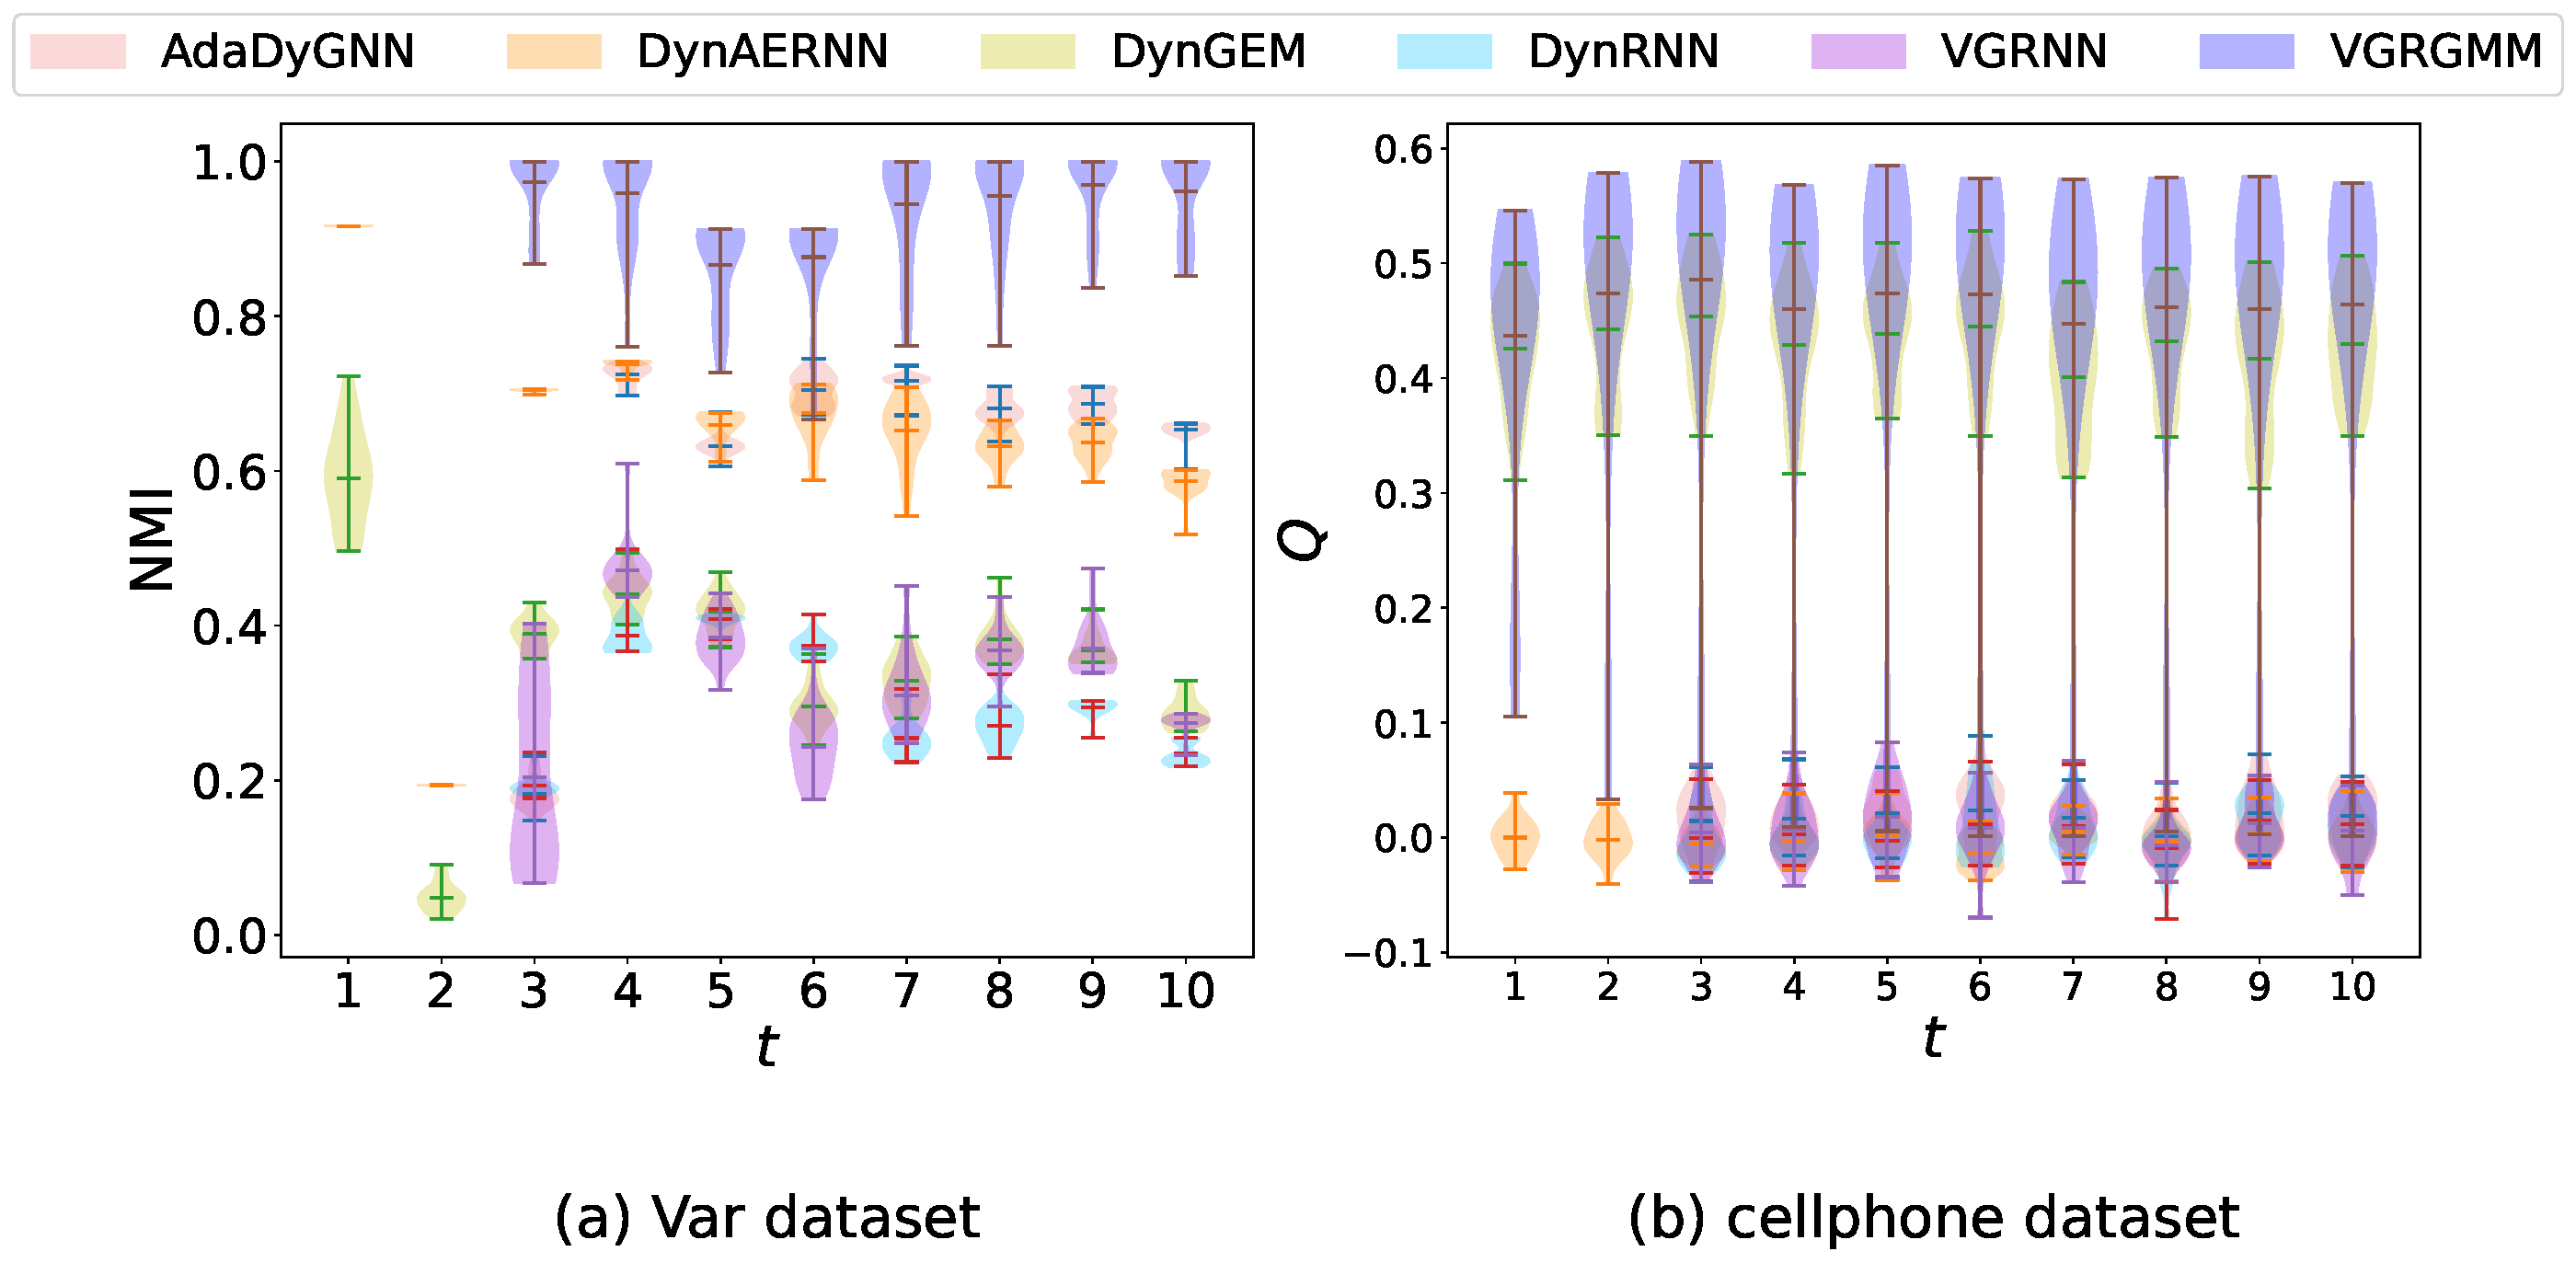
\includegraphics[width=.66\textwidth]{figures/chap06/chap5STNQ.pdf}
	\caption{模型稳定性对比小提琴图}
	\label{fig:STNQ}
\end{figure}

本节进一步利用cellphone数据对模型进行了鲁棒性测试,如图~\ref{fig:robustWP}所示,横坐标表示对cellphone随机抽取边的比例。随着网络的边被移除比例提升,网络的结构被破坏程度也越来越高。从图中可以看出,VGRGMM的鲁棒性随网络边的扰动变化不大,因模型的混合高斯先验能够很好地捕获数据分布,精准地刻画了网络的高阶生成机制(即社团结构 ),因此模型对网络噪声敏感性较低,具备良好的鲁棒性。
\begin{figure}[htbp]
	\centering
	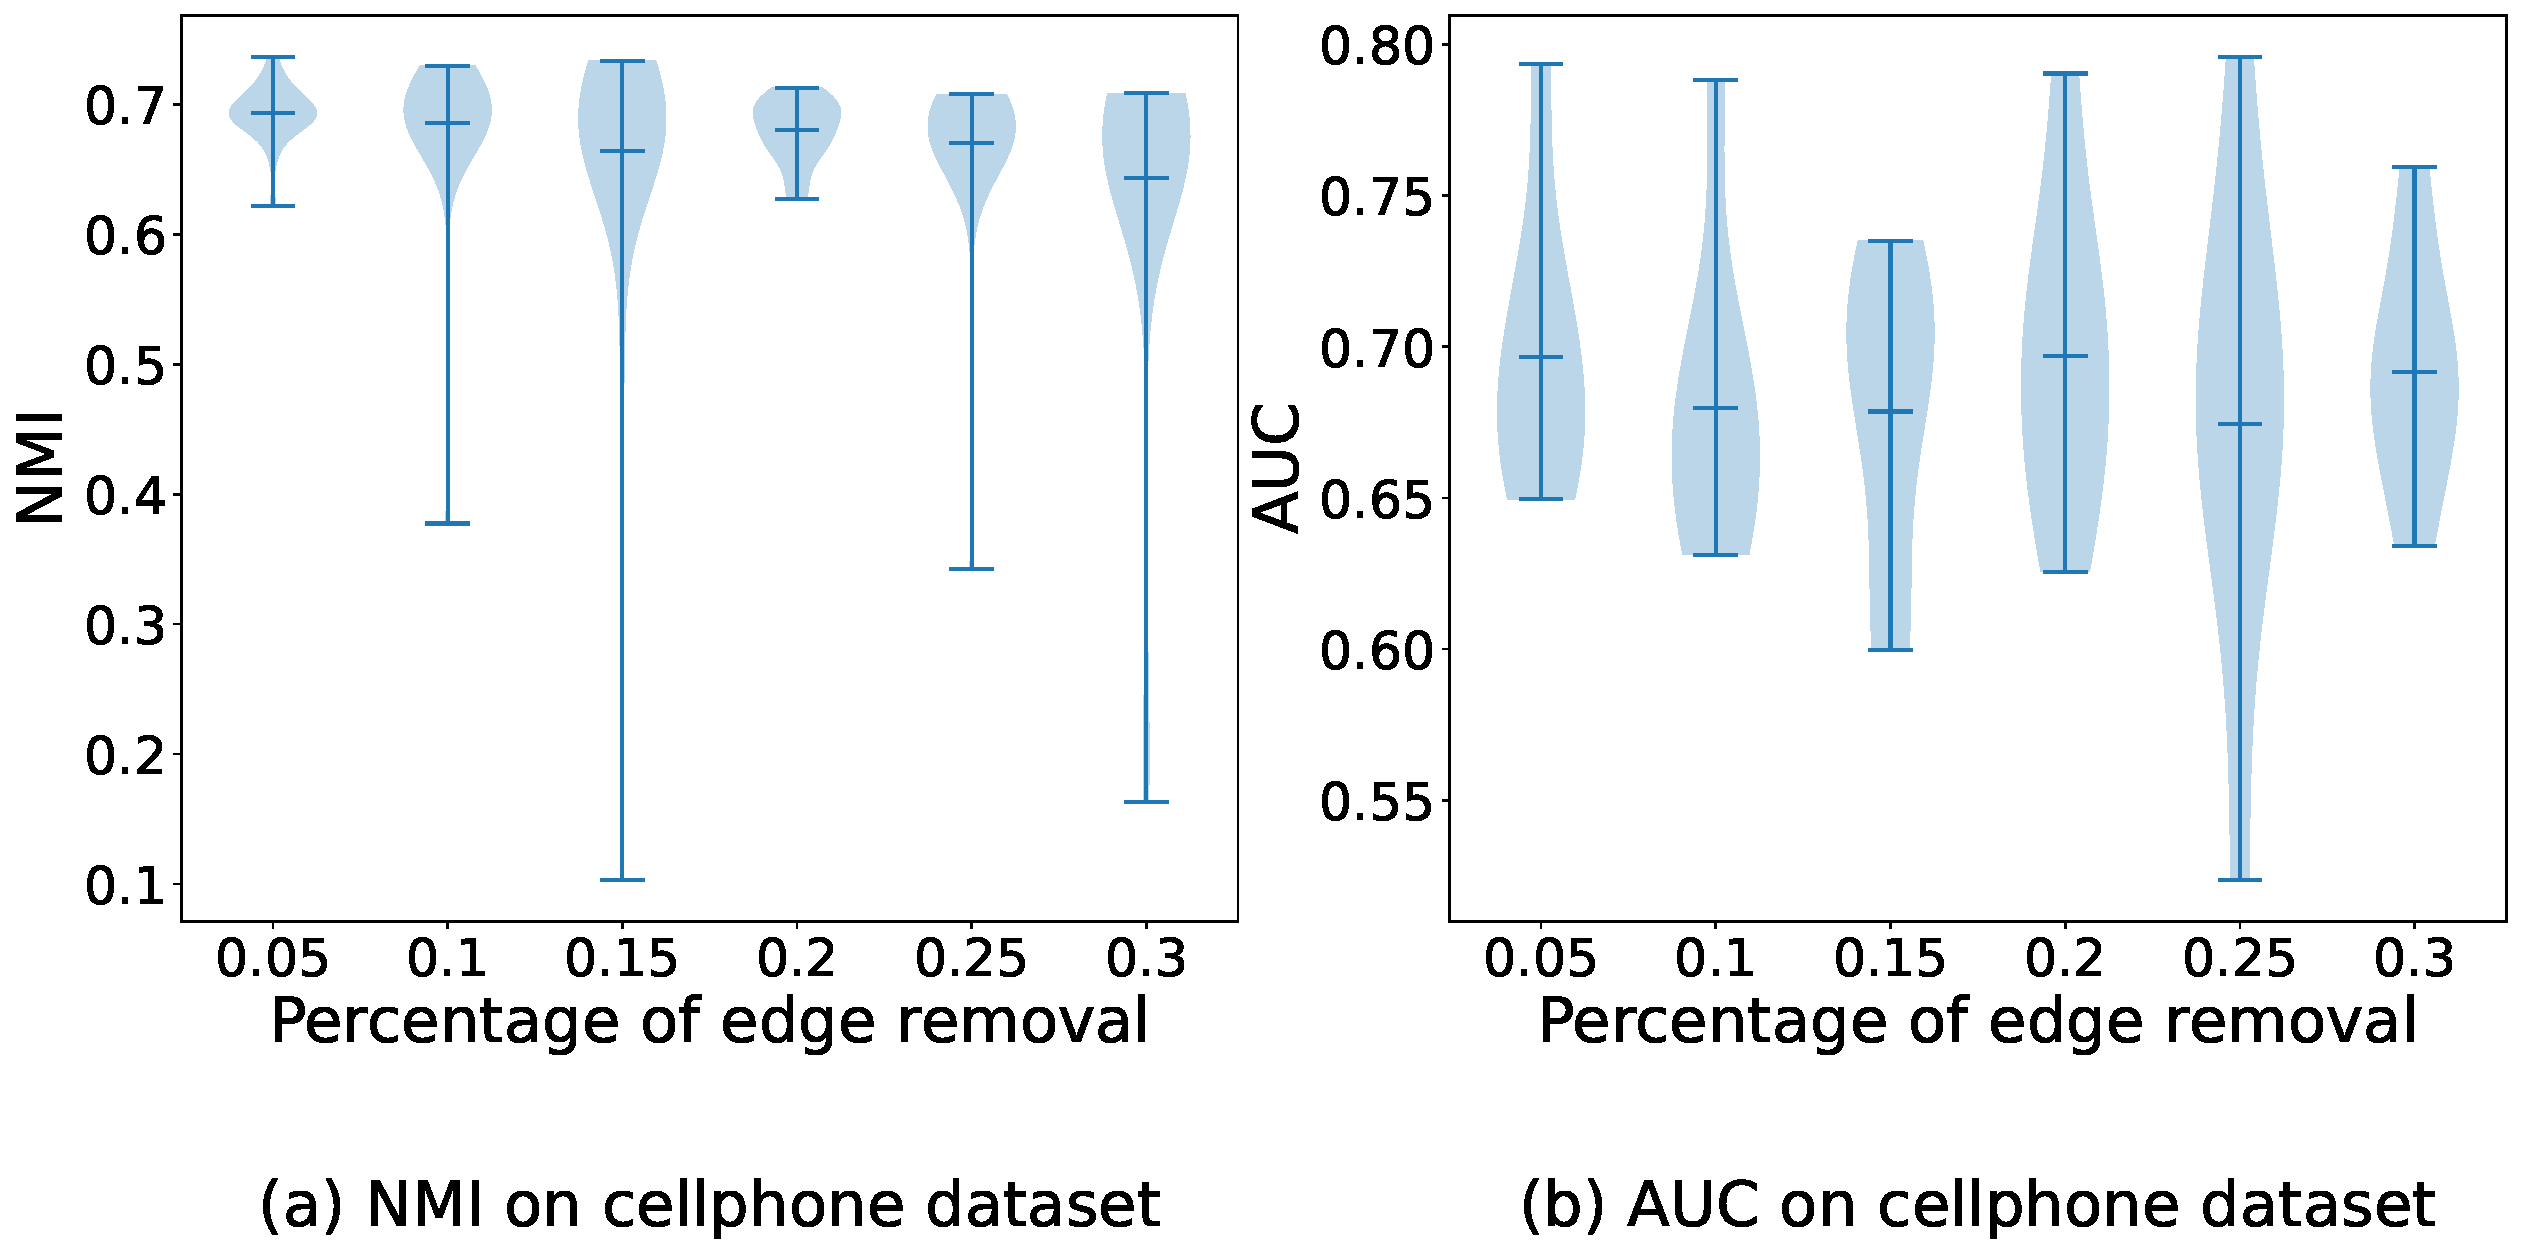
\includegraphics[width=.6\textwidth]{figures/chap06/workplaceRBNA.pdf}
	\caption{模型鲁棒性小提琴图}
	\label{fig:robustWP}
\end{figure}

\subsection{可视化结果}

\begin{figure}[htbp]
    \centering
    \subfigure[\small VGRGMM]{
    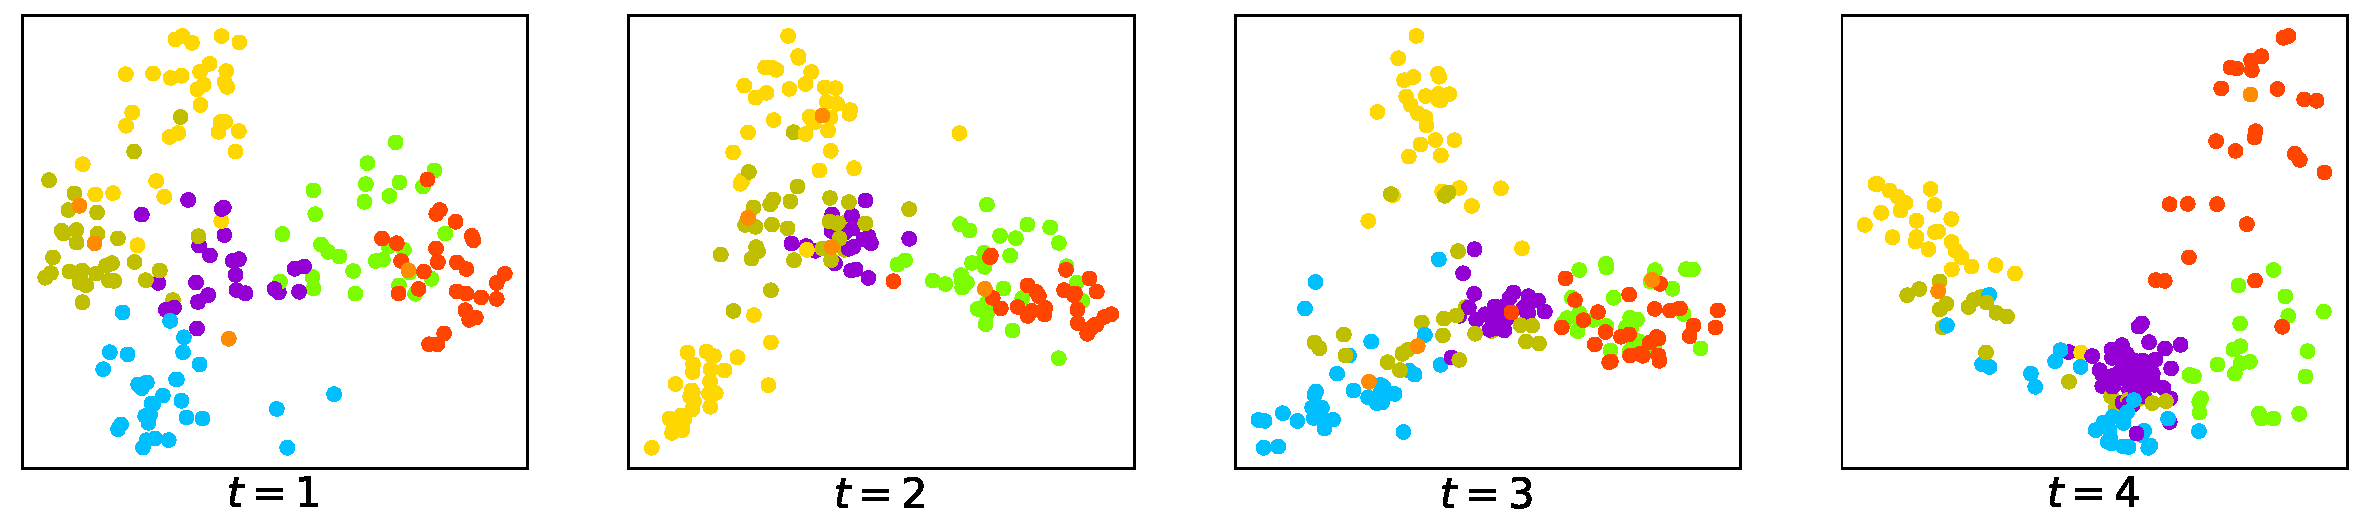
\includegraphics[width=.65\textwidth]{figures/chap06/ComDynVAE-HS12Visulization.pdf}
    }
    \subfigure[\small DynAERNN]{
    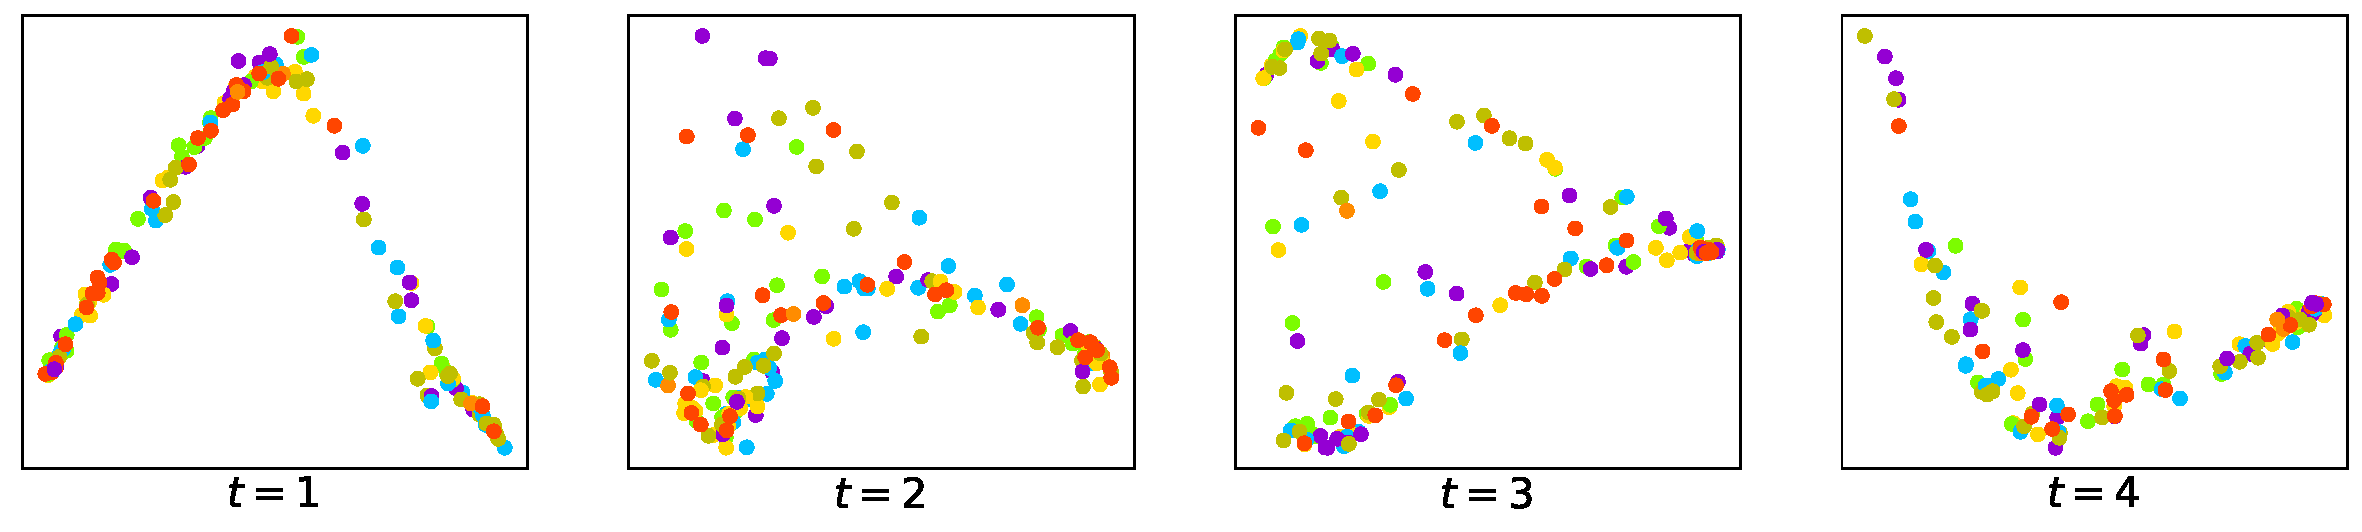
\includegraphics[width=.65\textwidth]{figures/chap06/DynAERNN-HS12Visulization.pdf}
    }
    \subfigure[\small VGRNN]{
    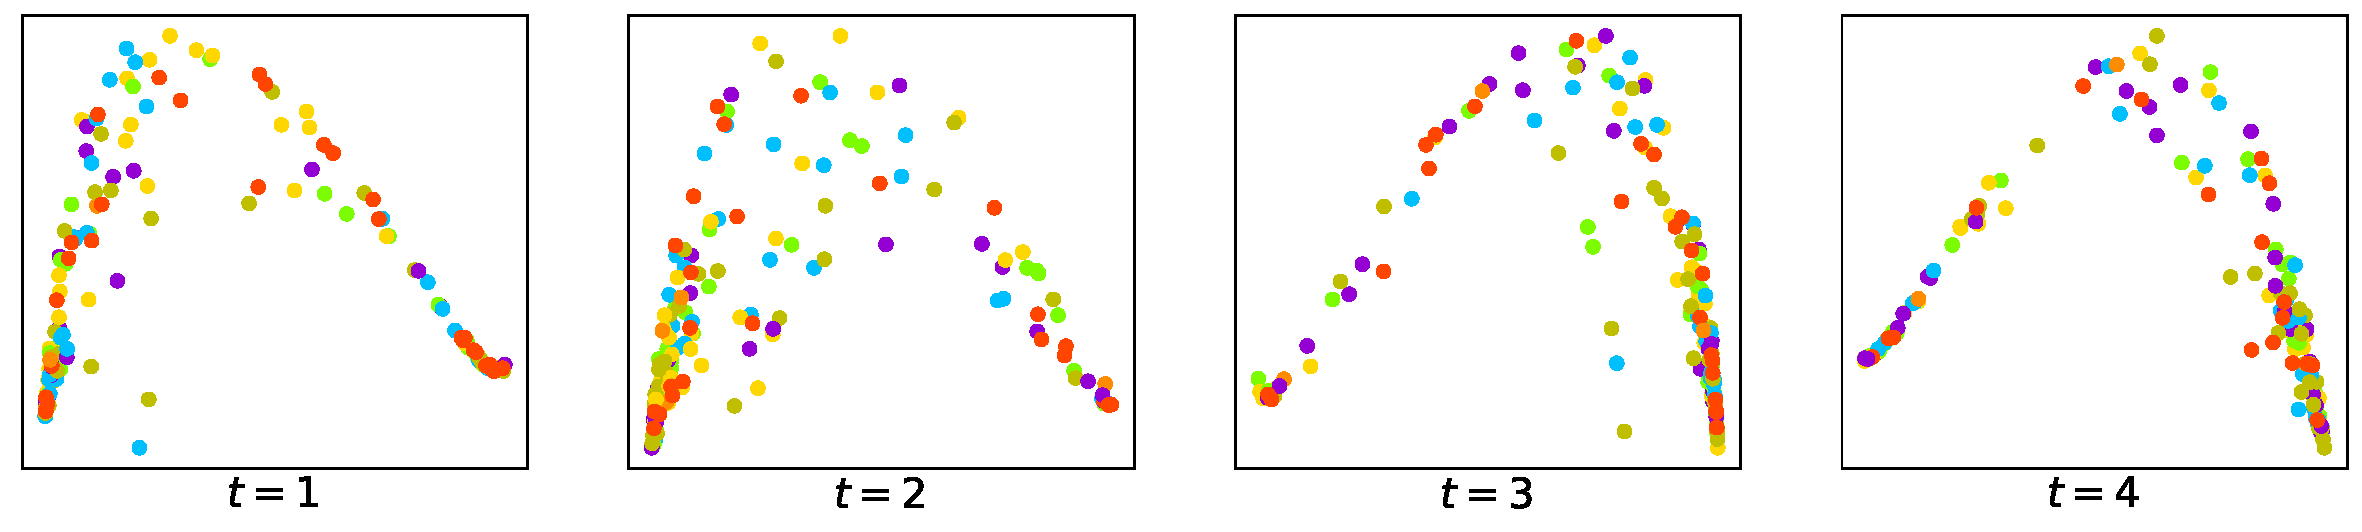
\includegraphics[width=.65\textwidth]{figures/chap06/DynRNN-HS12Visulization.pdf}
    }
    \caption{三种方法在HS12数据集中的表示向量高维可视化的结果}
    \label{fig:Visu}
\end{figure}

VGRGMM可以同时实现动态网络嵌入和社团检测任务,相较与传统动态网络表示学习方法,本方法的节点表示向量还包含了社团信息。这里通过将节点表示向量$Z$映射到二维欧几里得空间,展示了HS12数据集上节点表示的可视化结果。图~\ref{fig:Visu}展示了VGRGMM、DynAERNN和VGRNN在快照$t=1$到$t=4$中的tSNE可视化结果,同颜色节点表示其属于相同的社团。可以看到,由于引入了社团先验,VGRGMM中同一社团的节点表示比其他方法所检测社团的节点在高维空间中更接近。

此外,通过比较连续切片中的网络可视化结果,VGRGMM可以进一步分析社团的演化。例如,蓝色社团(左下角社团)是一个独立的社团,因为其节点在快照$t=1$和$t=2$中紧密聚集。然而,随着时间的推移,蓝色社团趋向于并入深黄色社团(快照$t=1$中最左边的社团),因为在快照$t=3$和$t=4$中,这两个社团的节点越来越接近。


\subsection{参数敏感性分析}




在本研究的模型VGRGMM中,除了嵌入维度$D$之外,没有其他额外的超参数。本研究分析了$D$对动态网络中社团检测结果的敏感性。本节选择了两个数据集,Primary和Enron数据集,分别使用\emph{NMI}和$Q$进行评估。如图~\ref{fig:Hyper} 所示,VGRGMM在两个网络中每个快照上$D$从$4$到$128$变化的结果。VGRGMM在节点表示向量维度为$32$时可以达到最佳性能。如果维度$D < 32$,则没有足够的维度来刻画网络结构。反之,当$D > 32$时,节点表示向量将对动态网络过拟合,因此在实验中设置$D = 32$。

\begin{figure}[htbp]
	\centering
	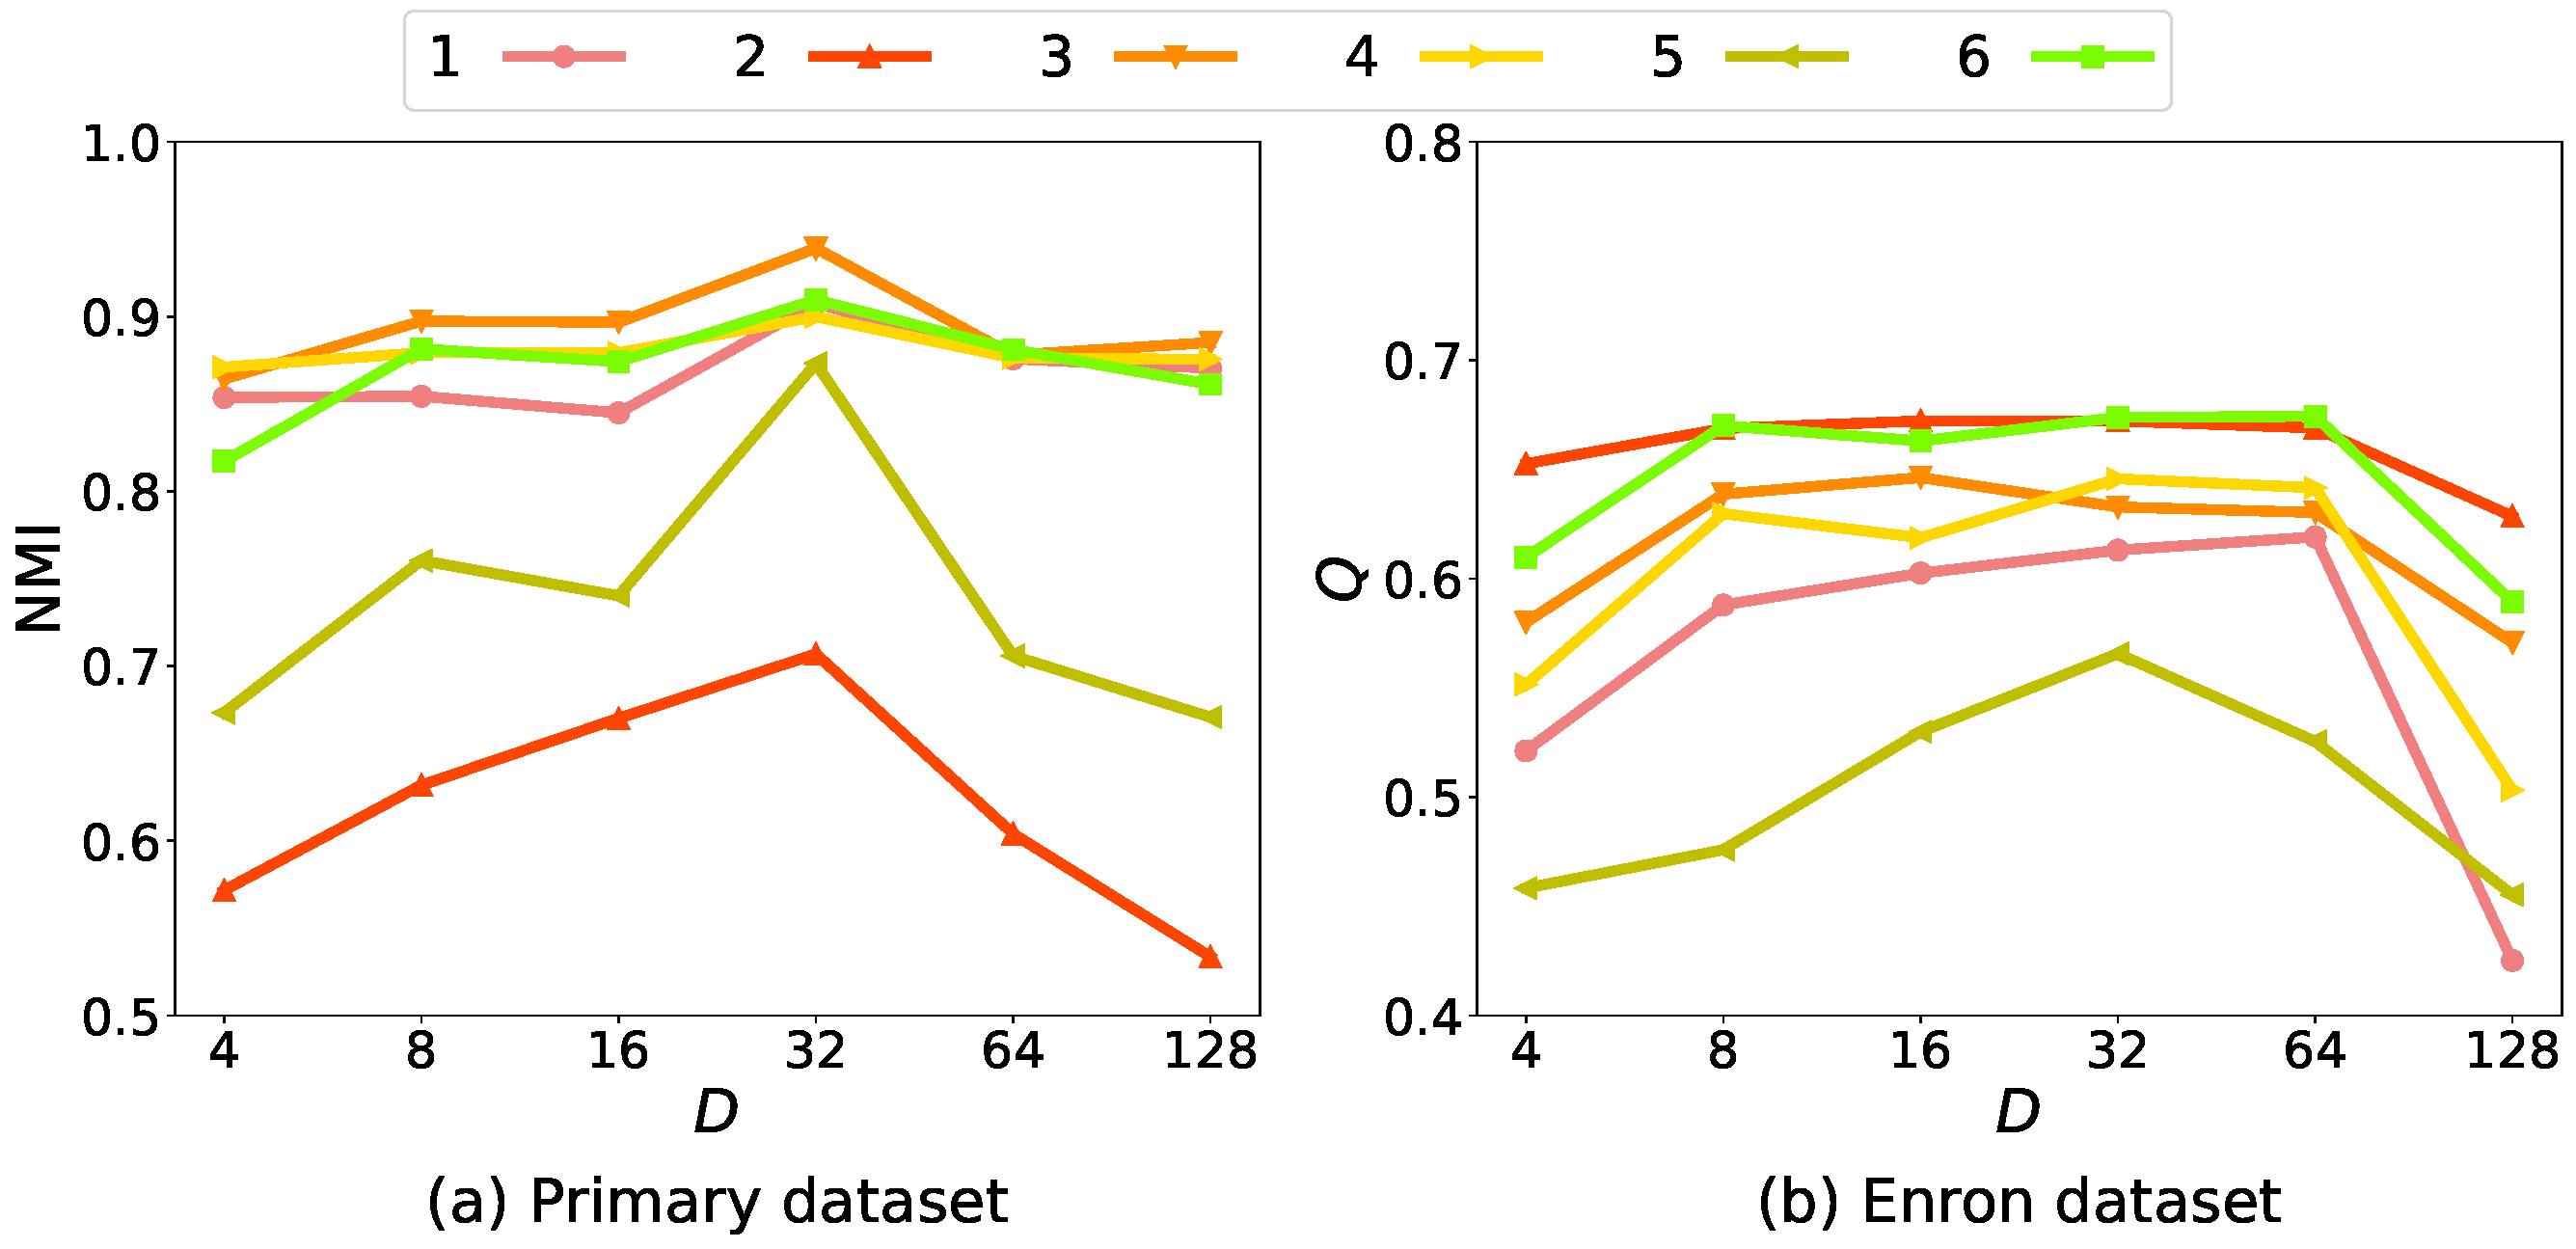
\includegraphics[width=.6\textwidth]{figures/chap06/DimensionsOndifferentData-t.pdf}
	\caption{VGRGMM 的参数敏感性分析}
	\label{fig:Hyper}
	\vspace{0cm}
\end{figure}




\subsection{实证分析}


最后,本章还展示了一个实证分析,以揭示VGRGMM在动态社团演化分析中的有效性。通过HS12动态社团检测,本节将VGRGMM和VGRNN的结果与快照$t=7$和$t=8$的社团真实值进行了比较。如图~\ref{fig:case} 所示,其可视化了两个连续快照中具有$5$个社团的子图的变化。在快照$7$中,VGRGMM几乎完美地识别了快照中的社团结构,而VGRNN则错误地划分了一些紫色节点的社团结果。从快照$t=7$到$t=8$的横向对比可以看出,红色社团发生了明显变化,一些节点加入了橙色社团(从图~\ref{fig:case} (a) 到 (d))。受这种节点社团演化的影响,VGRNN无法准确识别快照$8$的社团结果,例如节点$8$和$88$,反之,VGRGMM仍然实现了较准确的社团划分结果。
同时,从社团演化的角度(即纵向比较VGRGMM和VGRNN),VGRNN将太多属于红色社团的节点转移到其他社团,这与真实值不一致。


\begin{figure*}[htbp]
    \centering
    \subfigure[\small 真实值 $t=7$]{
        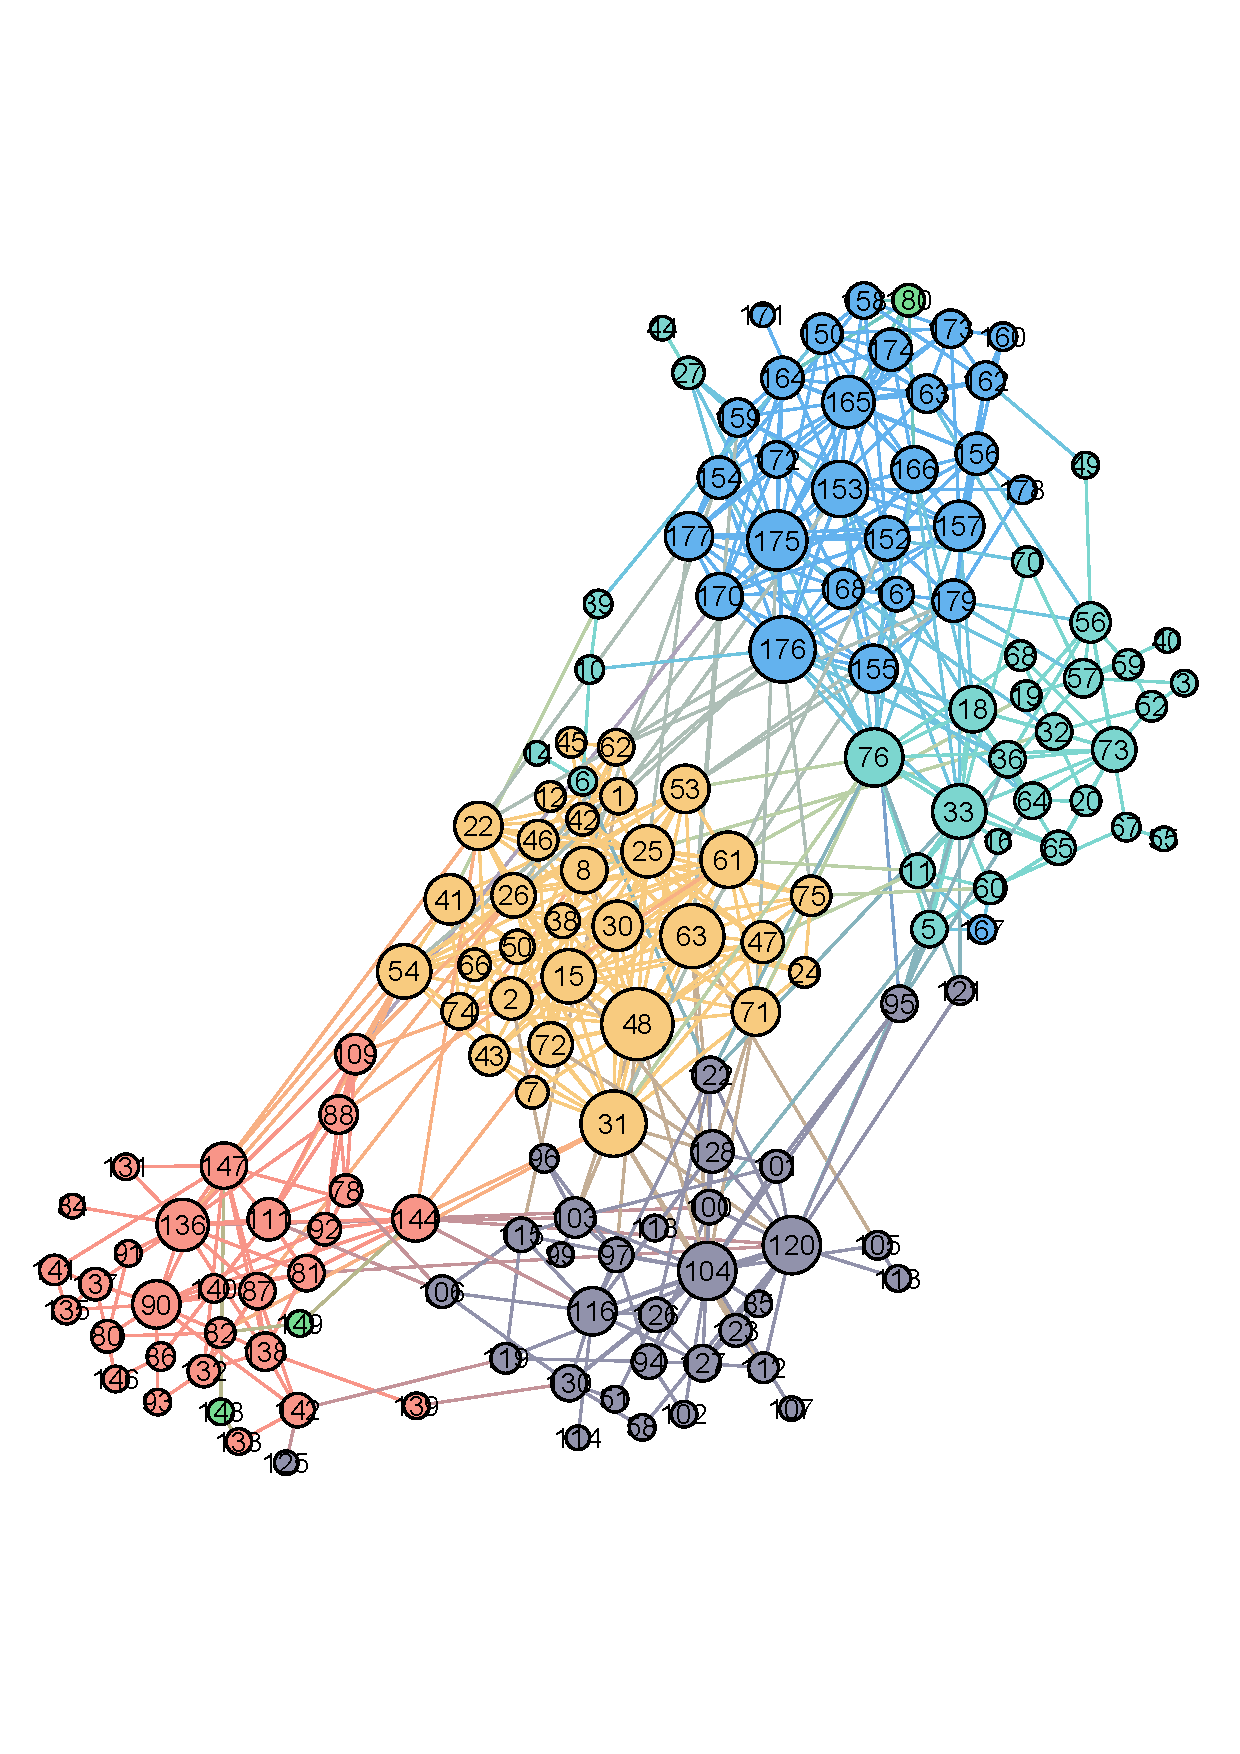
\includegraphics[width=.3\textwidth]{figures/chap06/g7truth.pdf}
    }
    \subfigure[\small VGRNN $t=7$]{
        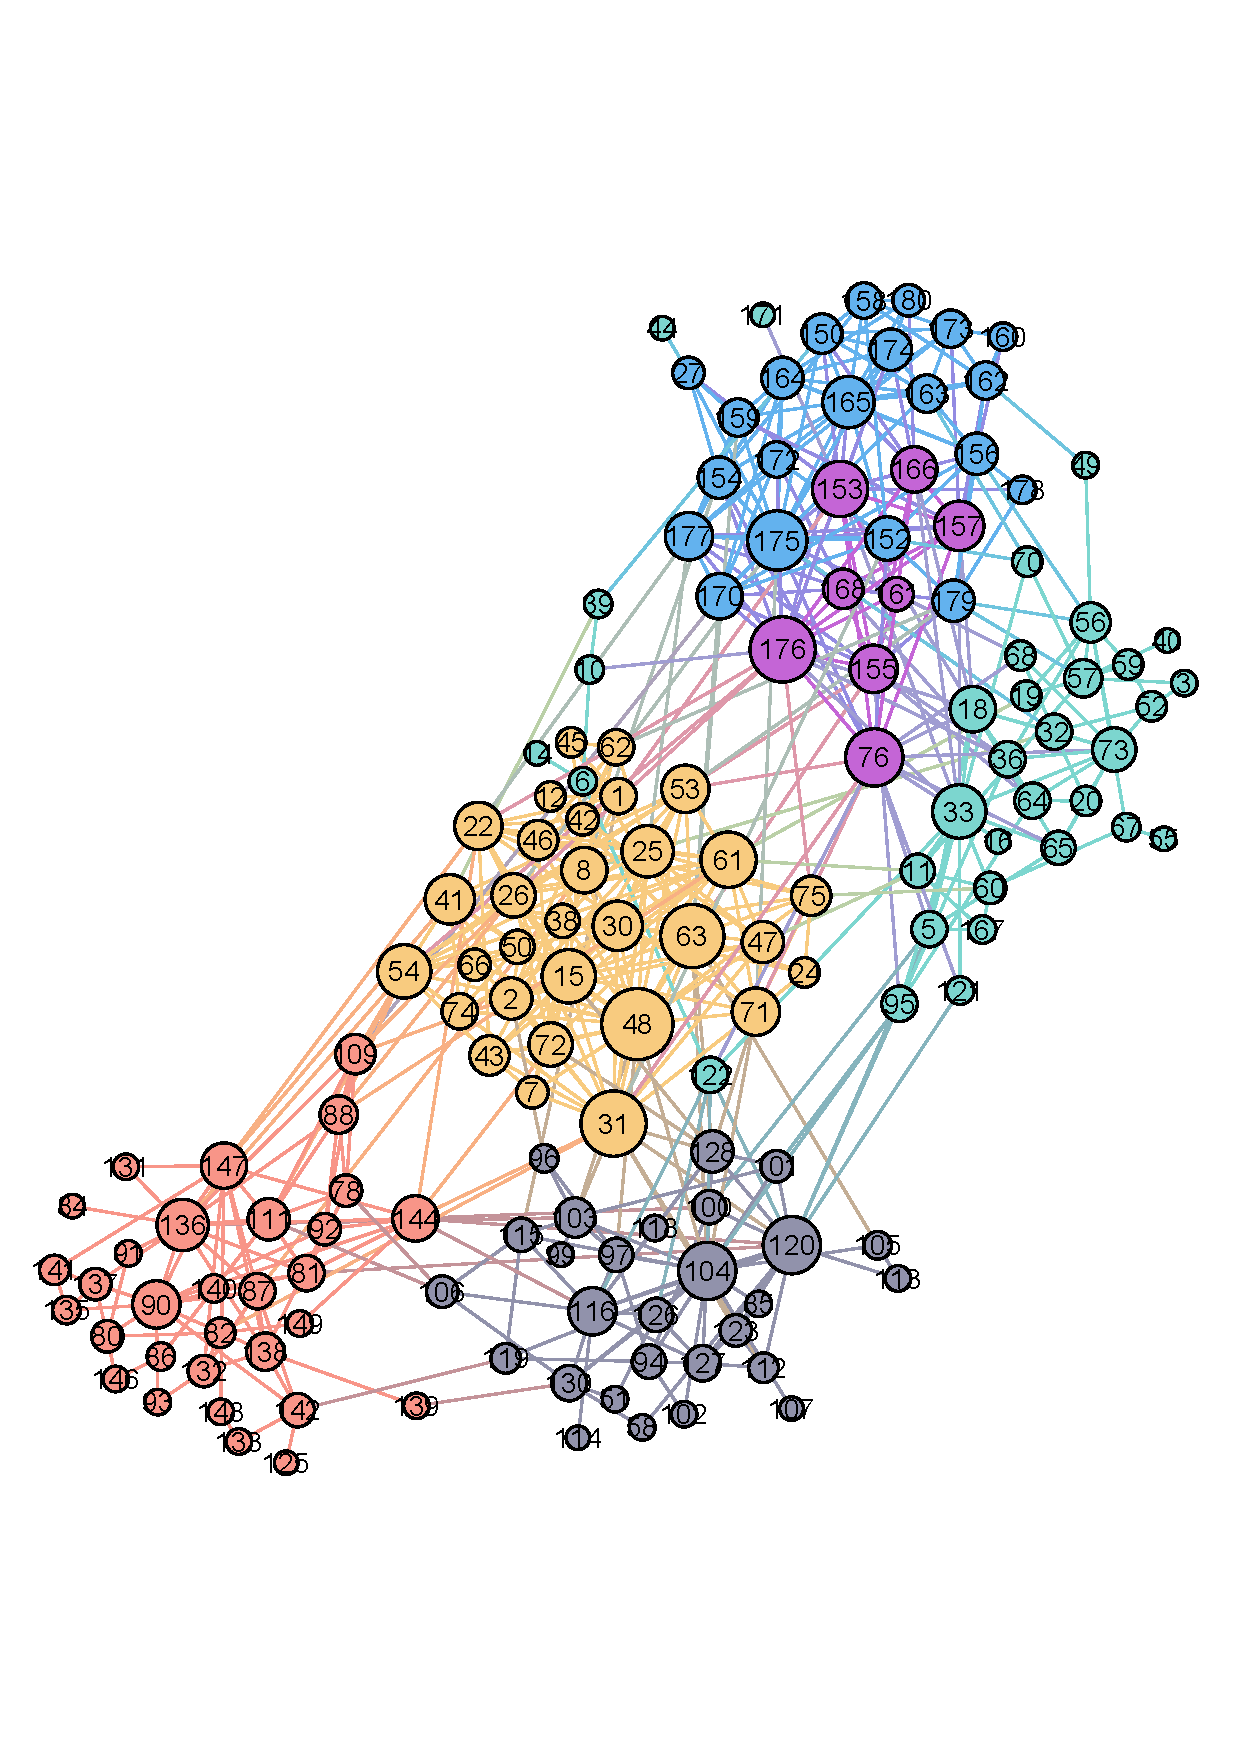
\includegraphics[width=.3\textwidth]{figures/chap06/g7VGMM.pdf}
    }
    \subfigure[\small VGRGMM $t=7$]{
        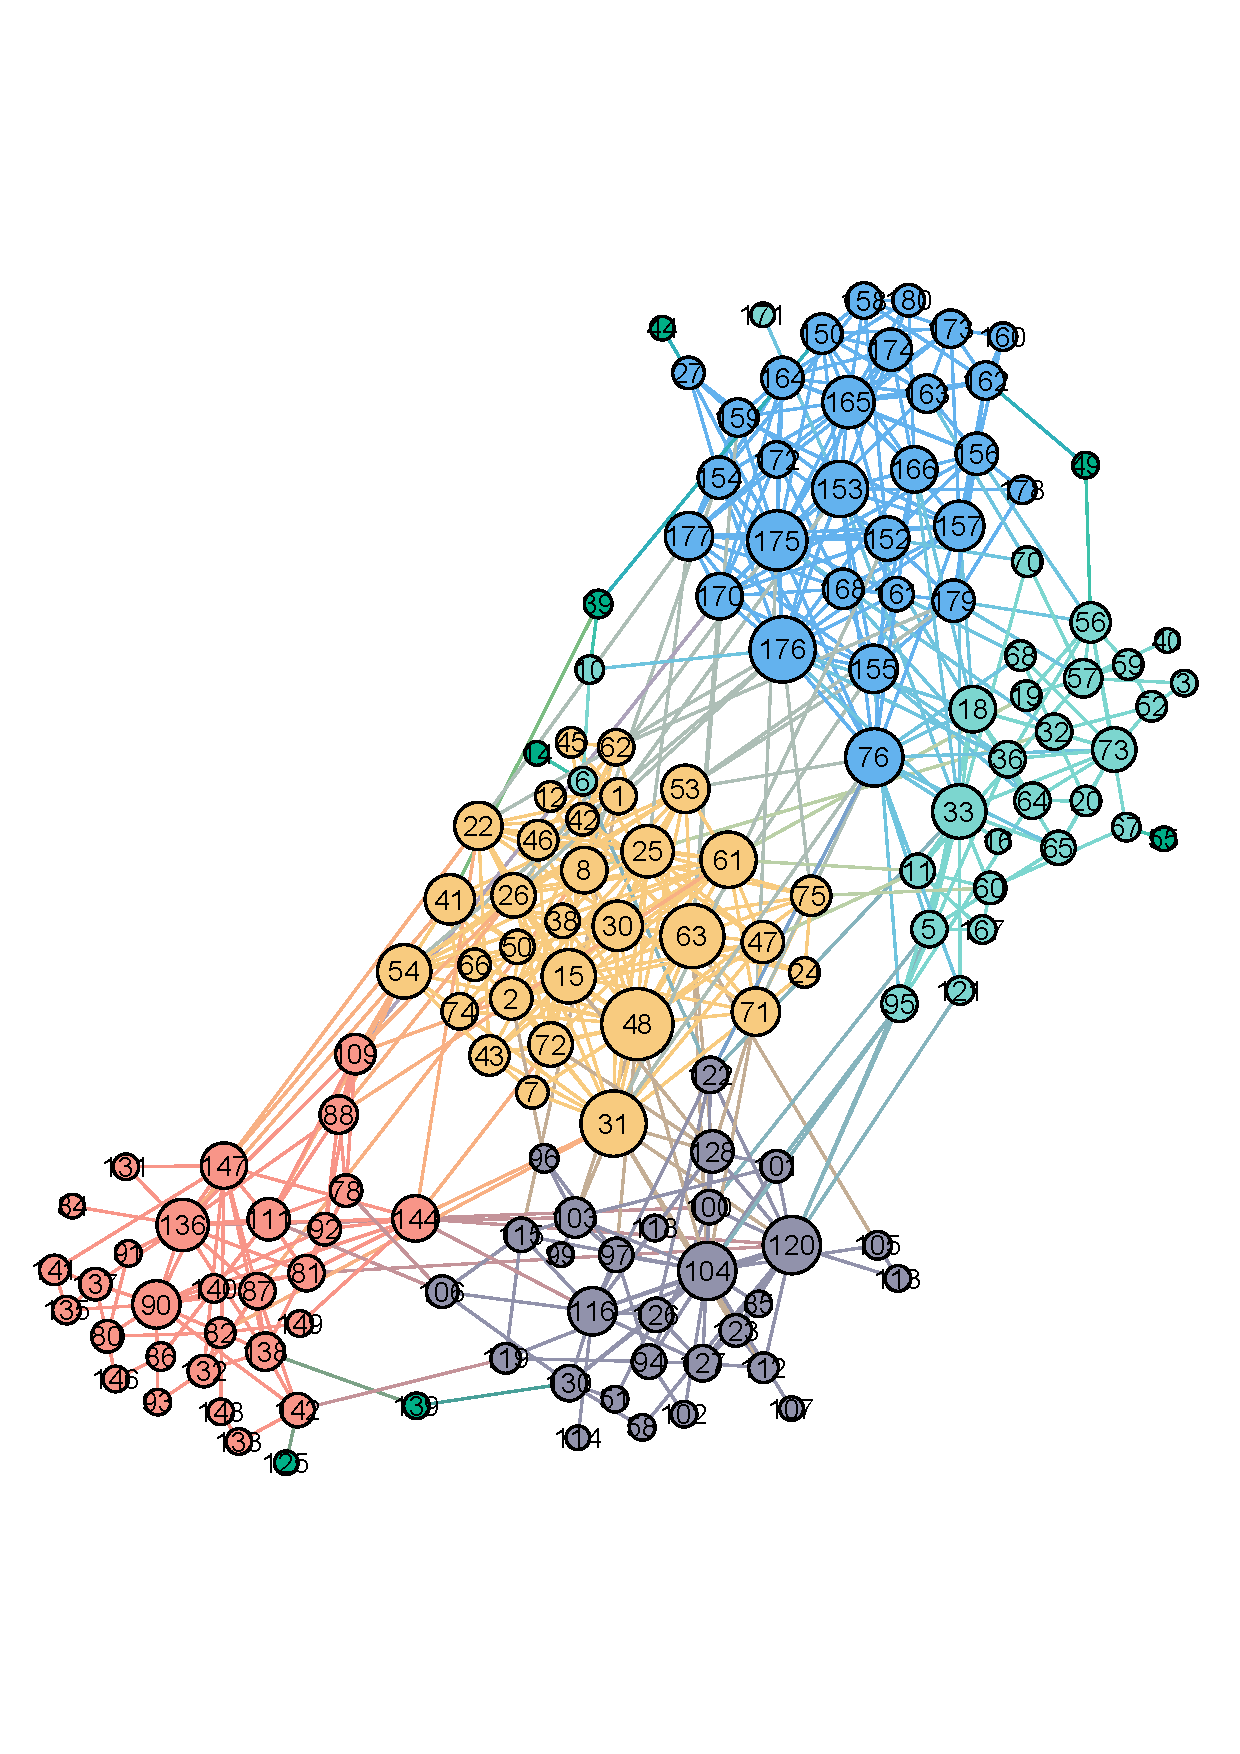
\includegraphics[width=.3\textwidth]{figures/chap06/g7VGRG.pdf}
    }
    \subfigure[\small 真实值 $t=8$]{
        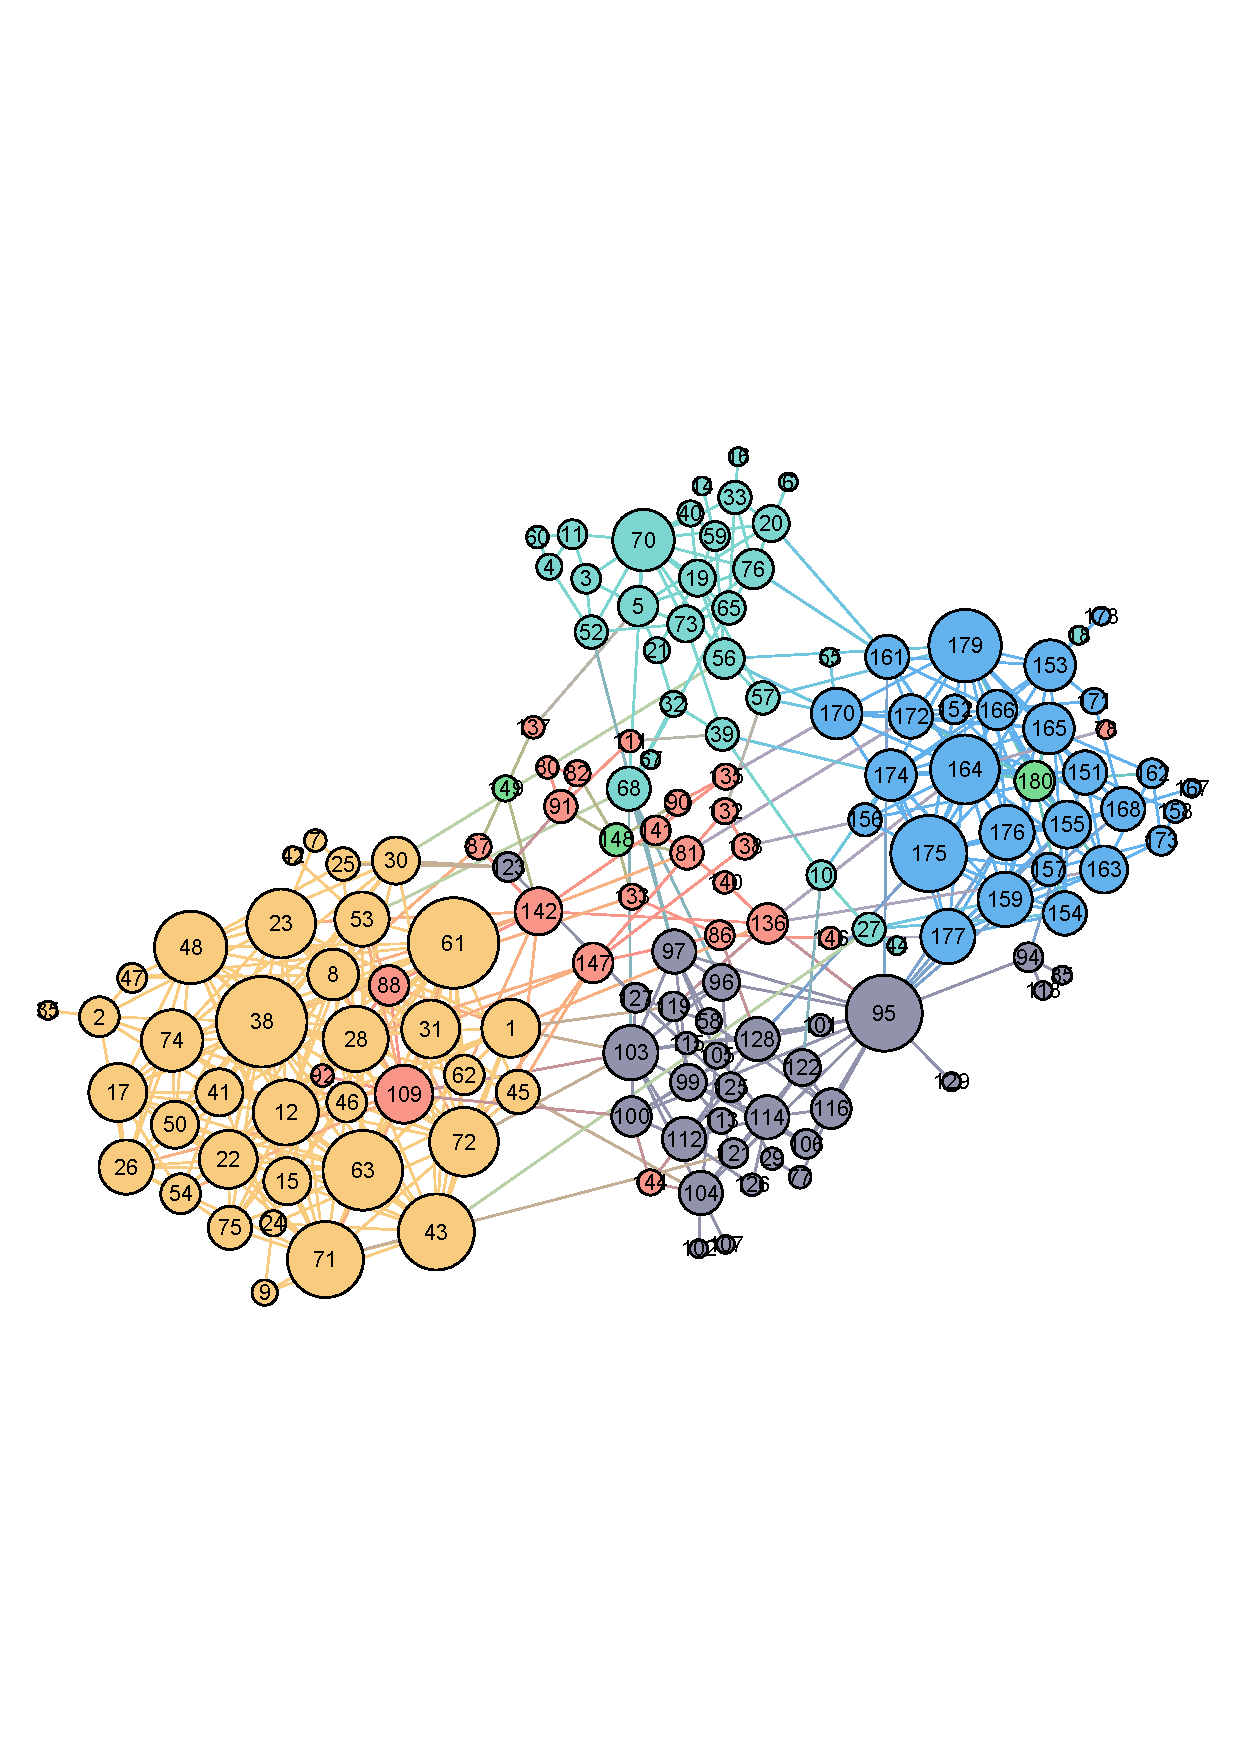
\includegraphics[width=.3\textwidth]{figures/chap06/g8truth.pdf}
    }
    \subfigure[\small VGRNN $t=8$]{
        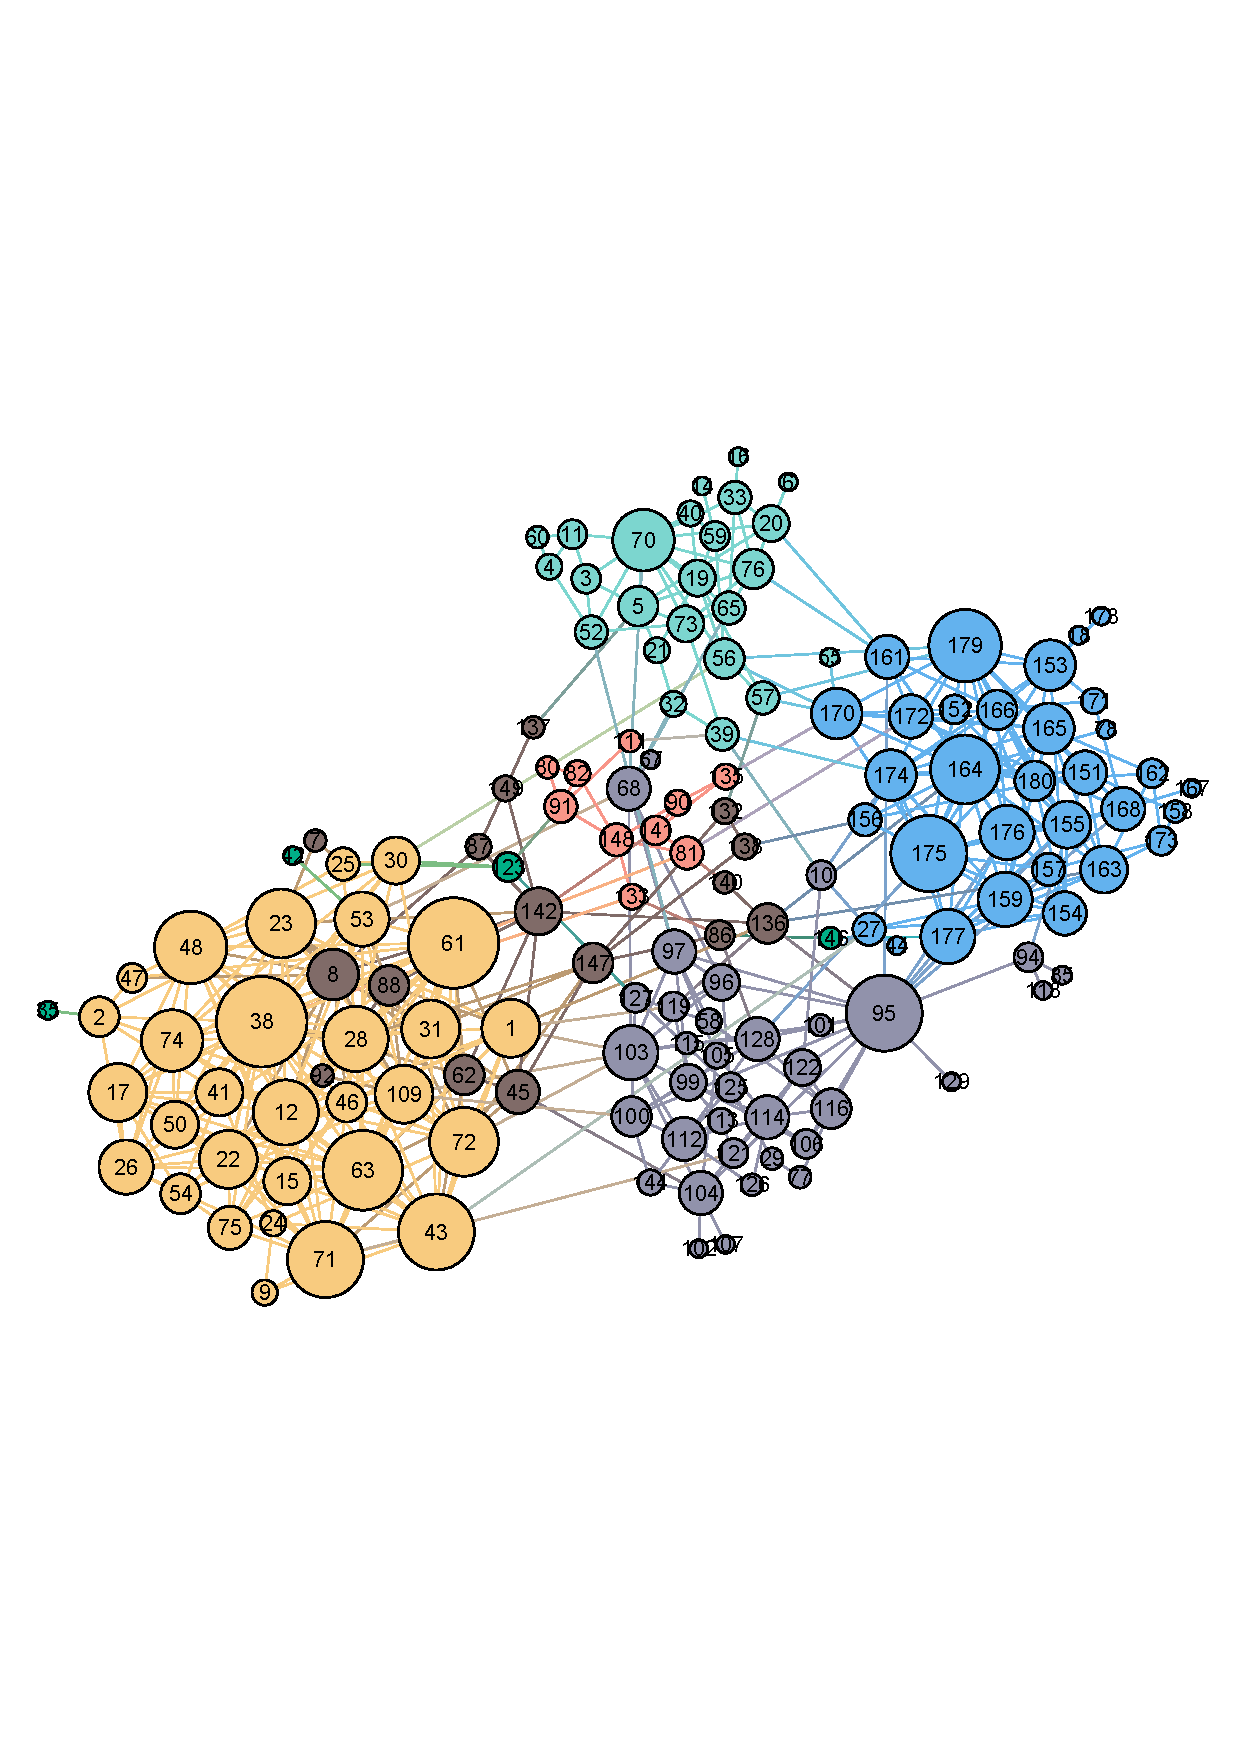
\includegraphics[width=.3\textwidth]{figures/chap06/g8VGMM.pdf}
    }
    \subfigure[\small VGRGMM $t=8$]{
        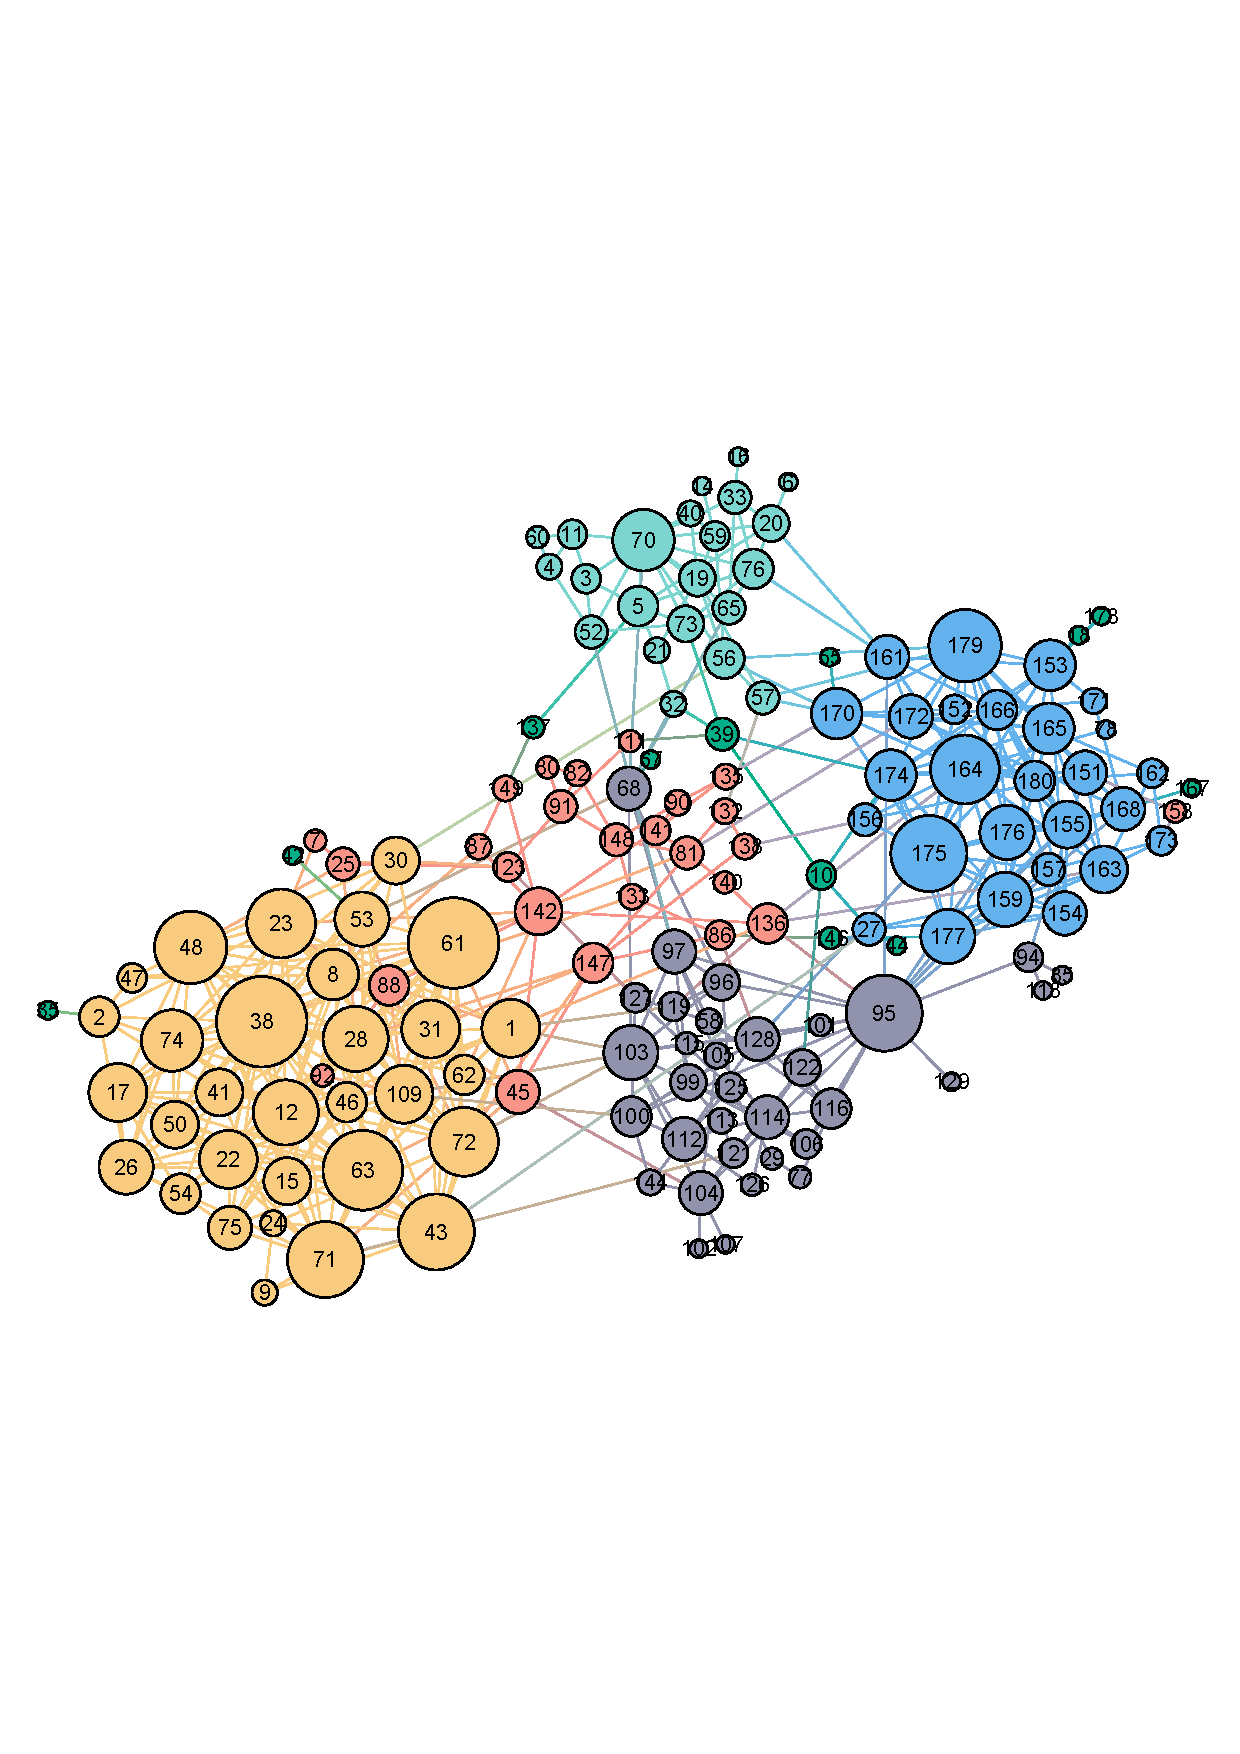
\includegraphics[width=.3\textwidth]{figures/chap06/g8VGRG.pdf}
    }
    \caption{HS12网络在快照$t=7$和$t=8$中子图的网络可视化,不同颜色代表不同的社团。}
    \label{fig:case}
\end{figure*}






\section{本章小结\label{chap6:summary}}
本章针对现有动态网络检测方法缺乏可解释性参数或无法建模大规模动态网络的问题,提出了基于变分图自编码器架构的深度动态网络社团检测算法VGRGMM。该模型首先利用变分图自编码器架构的基本设计,为深度学习模型引入了可解释可学习的参数,解决了深度模型的黑盒问题;其次,通过引入混合高斯先验,将动态网络的表示向量引入了社团结构信息,实现了对动态网络社团检测的神经网络化,提升了社团检测方法的运行效率;最后,利用改进的GRU模型刻画了动态网络的演化模式,并建模了动态网络的非线性变化,提升了模型的动态社团检测效果。实验证明了VGRGMM相较于传统社团检测算法与动态网络表示学习方法的“两步法”社团结构识别具有更好的动态社团检测效果,对各模型的运行效率实验也证明了本方法能够适应较大规模的动态网络数据。

但该模型仍然存在一定缺陷,首先,虽然VGRGMM成功地实现了对动态网络社团检测的深度建模,验证了深度生成模型在动态网络社团检测任务的有效性,但对于超大规模网络的计算仍然存在一定困难,因此需要进一步引入优化策略来实现模型对于超大模型的建模;其次,混合高斯先验的引入实现了动态网络社团检测与动态网络表示学习的结合,但前述章节的模型证明了动态网络的演化存在层次性,且其演化更加复杂,因此需要进一步将动态网络生成模型与动态网络表示学习进行结合以更好地建模动态网络的演化模式;最后,虽然可以利用该模型参数间接的实现对动态网络的演化分析,但模型本身对动态网络的非线性演化是通过GRU进行实现的,因此仍然存在模型黑盒难题,即无法可解释性地建模动态网络的演化。

%从动态网络下游任务的泛化能力看,虽然VGRGMM对于节点级别的任务能够通过节点表示向量的进一步分析进行统一,但子图或图级别的任务仍然难以统一。






